\chapter{Introduction}\label{french-introduction}
\graphicspath{{summary/figures/}}

\newcommand{\bi}{Business Intelligence }

La Business Intelligence (ou BI) a toujours \'{e}t\'{e} port\'{e} par la transformation des donn\'{e}es brutes en donn\'{e}es intelligibles. En donnant un sens aux donn\'{e}es, il est plus facile de conduire des changements dans les organisations. Un aspect cl\'{e} pour apporter du sens aux donn\'{e}es est d'attacher des informations pr\'{e}cises en lien avec les donn\'{e}es repr\'{e}sent\'{e}es. Cet aspect est \'{e}tudi\'{e} dans le domaine de la S\'{e}mantique.

La \bi ainsi que les nouveaux outils de visualisation agile concentrent une grande partie de leurs caract\'{e}ristiques de vente sur des repr\'{e}sentations visuelles attrayantes et uniques. La principale t\^{a}che, la plus ardue, est de pr\'{e}parer les donn\'{e}es pour ces outils de visualisation dans la plupart des projets de BI, petits ou grands. Ainsi, le but final de la BI est de simplifier la prise de d\'{e}cision en \'{e}liminant toute la lourdeur li\'{e}e \`{a} la gestion des syst\`{e}mes d'informations et des nombreuses donn\'{e}es collect\'{e}es. Traditionnellement, les approches BI sont g\'{e}r\'{e}es avec une version centralis\'{e}e et une s\'{e}paration distincte entre le monde du syst\`{e}me d'information et le monde de l'entreprise d\'{e}cisionnelle. La recherche des donn\'{e}es par l'utilisateur concern\'{e} apporte une solution pour rapprocher ces deux mondes et faciliter la capture et int\'{e}gration d'une mani\`{e}re intuitive pour l'utilisateur final.

\section{Contexte et Motivation}

Les entreprises utilisent un large panel de syst\`{e}mes d'information h\'{e}t\'{e}rog\`{e}nes dans leurs activit\'{e}s telles que la planification des ressources d'entreprise (ERP), de gestion des relations client (CRM) et de syst\`{e}mes de chaine d'approvisionnement (SCM). Un syst\`{e}me d'information distribu\'{e} contient plusieurs syst\`{e}mes utilisant diff\'{e}rentes briques technologies et plusieurs standards diff\'{e}rents~\cite{Mihindukulasooriya:COLD:13}. En plus de cette h\'{e}t\'{e}rog\'{e}n\'{e}it\'{e}, la quantit\'{e} d'information stock\'{e}e dans les bases de donn\'{e}es de l'entreprise et sur les diff\'{e}rents fournisseurs de stockage sur Internet augmente de fa\c{c}on exponentielle chaque ann\'{e}e. Ce qu'on appelle ``Enterprise Big Data'' n'est pas seulement corr\'{e}l\'{e} \`{a} un grand espace de stockage, mais aussi a une grande vari\'{e}t\'{e} dans les formats de fichiers associ\'{e}s. L'information est \'{e}galement souvent stock\'{e}es dans des formats non structur\'{e}s et inconnus.

L'int\'{e}gration des donn\'{e}es est un challenge. Elle n\'{e}cessite la combinaison de donn\'{e}es provenant de diff\'{e}rentes sources pour fournir \`{a} l'utilisateur une vue unifi\'{e}e de ces donn\'{e}es~\cite{Lenzerini:SIGMOD:02}. Dans les grandes entreprises, c'est une tache coûteuse en ressources et en temps. Diverses approches ont \'{e}t\'{e} propos\'{e}es pour r\'{e}soudre les probl\'{e}matiques d'int\'{e}gration. Ces approches ont \'{e}t\'{e} principalement bas\'{e}es sur XML comme syntaxe de repr\'{e}sentation de donn\'{e}es, les web-services en tant que protocole d'\'{e}change de donn\'{e}es et sur une architecture orient\'{e}e service (SOA) comme approche holistique de l'architecture de syst\`{e}mes distribu\'{e}s et de la communication. Cependant, il a \'{e}t\'{e} constat\'{e} que ces technologies ne sont pas suffisantes pour r\'{e}soudre les probl\`{e}mes d'int\'{e}gration dans les grandes entreprises~\cite{Frischmuth:ISWC:13,Frischmuth:SemWebJorunal:12}. R\'{e}cemment, des approches d'int\'{e}gration de donn\'{e}es bas\'{e}s sur l'ontologie ont \'{e}t\'{e} sugg\'{e}r\'{e}es, pour lesquels les ontologies sont utilis\'{e}es pour d\'{e}crire les donn\'{e}es, faire des requ\^{e}tes dessus et les synchroniser~\cite{Wache:IJCAI:01}. Une approche l\'{e}g\`{e}rement diff\'{e}rente est l'utilisation du concept de ``Linked Data''~\cite{Bizer:IJSWIS:09} pour l'int\'{e}gration de donn\'{e}es d'entreprise. Des entreprises comme Google et Microsoft utilisent ce paradigme pour l'int\'{e}gration de donn\'{e}es li\'{e}es \`{a} leurs syst\`{e}mes d'information, et elles vont encore plus loin en utilisant la technique pour construire des bases de connaissances compl\`{e}te (comme le Google Knowledge Graph aliment\'{e} en partie par Freebase\footnote{\url{http:// freebase .com}}) qui agissent comme un point central de leurs donn\'{e}es structur\'{e}es.

Les donn\'{e}es sont plus utiles quand elles sont ouvertes et largement diffus\'{e}es dans des formats partageables pour ensuite \^{e}tre le point de d\'{e}part d'analyses plus pouss\'{e}es. La qualit\'{e} et la quantit\'{e} de connaissance structur\'{e}e disponible sur le web rendent d\'{e}sormais possible pour les entreprises de parcourir cette \'{e}norme quantit\'{e} de donn\'{e}es publiques et de l'int\'{e}grer dans leurs syst\`{e}mes d'information de nouvelle g\'{e}n\'{e}ration. Un exemple de ce type de donn\'{e}es externe est l'initiative du Linked Open Data (LOD) disponible sur le cloud. En 2007, il y avait 12 bases de donn\'{e}es r\'{e}f\'{e}renc\'{e}es. Aujourd'hui, le catalogue contient plus de 1000 bases contenant plus de 82 milliards d'entrees\footnote{\url{http://datahub.io/dataset?tags=lod}}~\cite{Bizer:IJSWIS:09}. Les donn\'{e}es sont fournies aussi bien par des organismes publics que priv\'{e}s, et couvrent un ensemble diversifi\'{e} de domaines allant des sciences de la vie aux m\'{e}dias en passant par les donn\'{e}es du gouvernement. Le cloud LOD est potentiellement une mine d'or pour les organisations et les individus qui cherchent \`{a} tirer parti de sources de donn\'{e}es externes afin de produire des rapports plus \'{e}toff\'{e}s~\cite{Boyd:Article:11}. Ces donn\'{e}es externes peuvent \^{e}tre accessibles via des portails de donn\'{e}es publiques comme \texttt {datahub.io} et \texttt {publicdata.eu} ou priv\'{e}s comme \texttt{quandl.com} et \texttt{enigma.io}. L'analyse de ce nouveau type de donn\'{e}es dans le contexte des donn\'{e}es d'entreprise permet d'en tirer des analyses nouvelles ou plus pouss\'{e}es, ce qui permet de d\'{e}tecter et explorer de nouvelles opportunit\'{e}s de march\'{e}s~\cite{LaValle:MIT:11}.

\section{Sc\'{e}nario d'utilisation}

Pour permettre une int\'{e}gration efficace des donn\'{e}es \`{a} grande \'{e}chelle, il ya quelques efforts n\'{e}cessaires de en plusieurs points. Dans cette th\`{e}se, nous abordons les enjeux et les d\'{e}fis de deux points de vues :

\begin{itemize}
	\item \textbf{Analyste de donn\'{e}es :} Un analyste de donn\'{e}es est un professionnel exp\'{e}riment\'{e} qui est en mesure de recueillir et d'acqu\'{e}rir des donn\'{e}es provenant de multiples sources de donn\'{e}es, filtrer et nettoyer les donn\'{e}es, interpr\'{e}ter et analyser les r\'{e}sultats et fournir des rapports en cours.
	\item \textbf{Administrateur du portail de donn\'{e}es :} Un administrateur du portail de donn\'{e}es surveille la bonne tenue du portail. Il supervise la cr\'{e}ation des utilisateurs, des organisations et des ensembles de donn\'{e}es. Les administrateurs tentent d'assurer un niveau de qualit\'{e} de certaines donn\'{e}es en v\'{e}rifiant en permanence le spam, et en am\'{e}lioration manuellement les descriptions et annotations des ensembles de donn\'{e}es.
\end{itemize}

Tout au long de cette th\`{e}se, nous allons pr\'{e}senter un sc\'{e}nario de cas d'utilisation impliquant les deux personnes pour illustrer les d\'{e}fis et les solutions que nous fournissons.

Dans notre sc\'{e}nario, \textbf{Dan} est un analyste de donn\'{e}es en collaboration avec le minist\`{e}re charg\'{e} des Transports en France. Son outil de pr\'{e}dilection pour les calculs, la manipulation et la visualisation de donn\'{e}es est SAP Lumira\footnote{\url{http://saplumira.com/}}, un outil de visualisation de donn\'{e}es en libre-service qui le rend facile pour importer des donn\'{e}es provenant de sources multiples, effectuer une analyse BI visuelle \`{a} l'aide de tableaux de bord intuitifs, des cartes interactives, des graphiques, et des infographies. Dan re\c{c}oit une note de sa direction pour cr\'{e}er un rapport comparant le nombre d'accidents de voiture qui ont eu lieu en France pour cette ann\'{e}e, \`{a} son homologue du Royaume-Uni (UK). En outre, il est demand\'{e} de mettre en \'{e}vidence les accidents li\'{e}s \`{a} la consommation ill\'{e}gale d'alcool dans les deux pays.

Apr\`{e}s avoir examin\'{e} les dossiers du minist\`{e}re, Dan est en mesure de recueillir les donn\'{e}es n\'{e}cessaires pour cr\'{e}er son rapport pour la partie française. Dan publie \'{e}galement une demande officielle au minist\`{e}re des Transports au Royaume-Uni pour collecter les donn\'{e}es n\'{e}cessaires. Cependant, Dan sait que le processus prend beaucoup de temps alors qu'il doit rendre le rapport sous quelques jours. Dan est familier avec le mouvement Open Data et commence son voyage \`{a} travers diff\'{e}rents portails de recherche de donn\'{e}es au Royaume-Uni.

\textbf{Paul} est un administrateur du portail de donn\'{e}es pour le \texttt{data.gov.uk}. Il supervise en permanence les processus d'acquisition, et il pr\'{e}pare et publie des ensembles de donn\'{e}es. Paul essaie toujours de veiller \`{a} ce que les donn\'{e}es publi\'{e}es soient de haute qualit\'{e} et contiennent des m\'{e}tadonn\'{e}es attach\'{e}es suffisantes pour permettre une recherche et d\'{e}couverte simple. Paul re\c{c}oit souvent des plaintes au sujet des ensembles de donn\'{e}es inexacts ou de spam. Il supprime manuellement et corrige les erreurs tout en gardant les canaux de communication ouverts avec les diff\'{e}rents d\'{e}partements lui fournissant des donn\'{e}es.

%%%%%%%%%%%%%%%%%%%%%%%%%
%%% Research Challenges %%%
%%%%%%%%%%%%%%%%%%%%%%%%%

\section{Probl\'{e}matiques de Recherche}

Dans le sc\'{e}nario pr\'{e}sent\'{e} ci-dessus, les fournisseurs de donn\'{e}es (administrateurs du portail) et les utilisateurs (analystes de donn\'{e}es) ont besoin de solutions pragmatiques qui les aident dans leurs t\^{a}ches. Pour permettre cela, il y a quelques probl\'{e}matiques de recherche difficiles qui doivent \^{e}tre abord\'{e}es. Ces d\'{e}fis sont organis\'{e}s en trois cat\'{e}gories comme suit :

\subsection{Int\'{e}gration et Am\'{e}lioration des Donn\'{e}es}

\begin{itemize}
\item La diversit\'{e} des sources de donn\'{e}es en entreprise soul\`{e}ve de grandes probl\'{e}matiques. Il y a de nombreux formats de fichiers diff\'{e}rents, des protocoles d'acc\`{e}s ainsi que des langages de requ\^{e}te vari\'{e}s. Les sources de donn\'{e}es poss\`{e}dent leur propre mod\`{e}le de donn\'{e}es avec diff\'{e}rentes façons de repr\'{e}senter et stocker les donn\'{e}es. Ces donn\'{e}es \`{a} travers ces sources peuvent \^{e}tre incompl\`{e}tes, incompatibles, ou redondantes. Aussi, elles peuvent sembler s\'{e}mantiquement similaire mais pourtant diff\'{e}rentes.\textbf{Paul} a besoin d'outils puissants pour cartographier et organiser les donn\'{e}es afin d'avoir une vue unifi\'{e}e pour ces structures de donn\'{e}es h\'{e}t\'{e}rog\`{e}nes et complexes.
\item L'ajout de m\'{e}tadonn\'{e}es et d'informations s\'{e}mantiques peut \^{e}tre d\'{e}licat. Une entit\'{e} n'est g\'{e}n\'{e}ralement pas associ\'{e}e \`{a} un type g\'{e}n\'{e}rique unique dans la base de connaissances, mais plut\^{o}t \`{a} un ensemble de types sp\'{e}cifiques qui peuvent \^{e}tre pertinents ou non compte tenu du contexte. \textbf{Paul} se doit de trouver le type de l'entit\'{e} la plus pertinente dans un contexte donn\'{e}.
\item Les entit\'{e}s jouent un r\^{o}le cl\'{e} dans les bases de connaissances en g\'{e}n\'{e}ral et dans le Web des donn\'{e}es en particulier. Les entit\'{e}s comme celles de DBpedia, sont g\'{e}n\'{e}ralement d\'{e}crites avec beaucoup de propri\'{e}t\'{e}s. Cependant, il est difficile pour \textbf{Dan} d'\'{e}valuer celles qui sont plus ``importantes'' que d'autres pour des tâches particuli\`{e}res telles que la visualisation des principales caract\'{e}ristiques d'une entit\'{e}.
\item Les r\'{e}seaux sociaux ne sont pas seulement un rassemblement des utilisateurs d'Internet en groupes d'int\'{e}r\^{e}ts communs. Ils aident aussi les gens \`{a} s'informer des d\'{e}p\^{e}ches, \`{a} contribuer aux d\'{e}bats en ligne ou apprendre des autres. Ils sont en train de transformer l'utilisation du Web en se positionnant comme point d'entr\'{e}e principal dans la recherche, la navigation et l'analyse du comportement d'achat. Cependant, l'int\'{e}gration des informations de ces r\'{e}seaux sociaux peut \^{e}tre difficile \`{a} \textbf{Paul} en raison de la grande quantit\'{e} de donn\'{e}es disponibles. Il est plus difficile de rep\'{e}rer ce qui est pertinent en temps opportun.
\end{itemize}

\subsection{Maintenance et D\'{e}couverte des Donn\'{e}es}

\begin{itemize}
\item M\^{e}me si les ensembles de donn\'{e}es populaires comme DBPedia\footnote{\url{http://dbpedia.org}} et Freebase sont bien connus et largement utilis\'{e}s, il existe d'autres sources de donn\'{e}es plus cach\'{e}es qui ne sont pas utilis\'{e}es. En effet, ces ensembles de donn\'{e}es peuvent \^{e}tre utiles pour les domaines sp\'{e}cialis\'{e}s, mais sans maintenance d'annuaire pr\'{e}cis sur les sujets, il est difficile pour les analystes de donn\'{e}es comme \textbf{Dan} de les trouver~\cite{Lalithsena:WI:13}.
\item La quantit\'{e} croissante de donn\'{e}es n\'{e}cessite des m\'{e}tadonn\'{e}es riches pour atteindre son plein potentiel. Ces m\'{e}tadonn\'{e}es permettent la d\'{e}couverte de donn\'{e}es, la compr\'{e}hension, l'int\'{e}gration et la maintenance de ces donn\'{e}es. Malgr\'{e} les diff\'{e}rents mod\`{e}les et des vocabulaires d\'{e}crivant les ensembles de donn\'{e}es, la possibilit\'{e} d'avoir une compr\'{e}hension de l'ensemble des donn\'{e}es en inspectant seulement les m\'{e}tadonn\'{e}es peut \^{e}tre limit\'{e}e. Par exemple, \textbf{Dan} a des difficult\'{e}s \`{a} trouver des ensembles de donn\'{e}es avec une couverture g\'{e}ographique sp\'{e}cifique, car cette information est manquante \`{a} partir de presque tous les profils de jeux de donn\'{e}es examin\'{e}s.
\item Les utilisateurs, les organisations et les gouvernements sont habilit\'{e}s \`{a} publier des ensembles de donn\'{e}es. Toutefois, les administrateurs du portail de donn\'{e}es comme \textbf{Paul} ont besoin de v\'{e}rifier en permanence et manuellement la qualit\'{e} de ces publications pour d\'{e}tecter le spam et maintenir une haute qualit\'{e} de service.
\end{itemize}

\subsection{Qualit\'{e} des Donn\'{e}es}

Les donn\'{e}es li\'{e}es (Linked Data) utilisent de l'information structur\'{e}e d\'{e}crite par des mod\`{e}les, des ontologies et des vocabulaires, et elles contiennent des liens et des destinations pour effectuer des requ\^{e}tes. L'ensemble de ces informations rend la coh\'{e}rence, et donc la qualit\'{e} des donnes difficile \`{a} maintenir. Malgr\'{e} le fait que la tendance et la demande est tr\`{e}s forte autour de la qualit\'{e} des donn\'{e}es publiques li\'{e}es (Linked Open Data), tr\`{e}s peu d'initiatives sont initi\'{e}es pour essayer de normaliser et de formaliser des processus. Ainsi, il n'existe pas de scores ou de certificats permettant d'aider les d\'{e}cisionnaires quant \`{a} la pertinence et qualit\'{e} des donn\'{e}es. Les administrateurs de portail de donn\'{e}es comme \textbf{Paul} ont besoin d'avoir une vision globale de la qualit\'{e} de leurs portails. Ils voudraient ainsi int\'{e}grer ces param\`{e}tres dans les profils de leur source de donn\'{e}es existantes. D'autre part, les analystes de donn\'{e}es et les utilisateurs comme \textbf{Dan} veulent savoir \`{a} l'avance si l'ensemble de donn\'{e}es est d'un certain niveau de qualit\'{e} pour \^{e}tre utilis\'{e} dans leurs rapports.

%%%%%%%%%%%%%%%%%%%%%%%%%
%%% Thesis Contributions %%%
%%%%%%%%%%%%%%%%%%%%%%%%%

\section{Contributions de la Th\`{e}se}

Dans cette th\`{e}se, nous proposons un ensemble d'outils pour permettre l'acc\`{e}s \`{a} des donn\'{e}es en libre-service pour des sources internes et externes \`{a} l'entreprise. Les outils contribuent aux trois principales probl\'{e}matiques d\'{e}crites ci-dessus. En r\'{e}sum\'{e}, les principales contributions de ce travail sont les suivantes :

\begin{adjustwidth}{-.4in}{-.4in}
\begin{figure}[!ht]
	\centering
	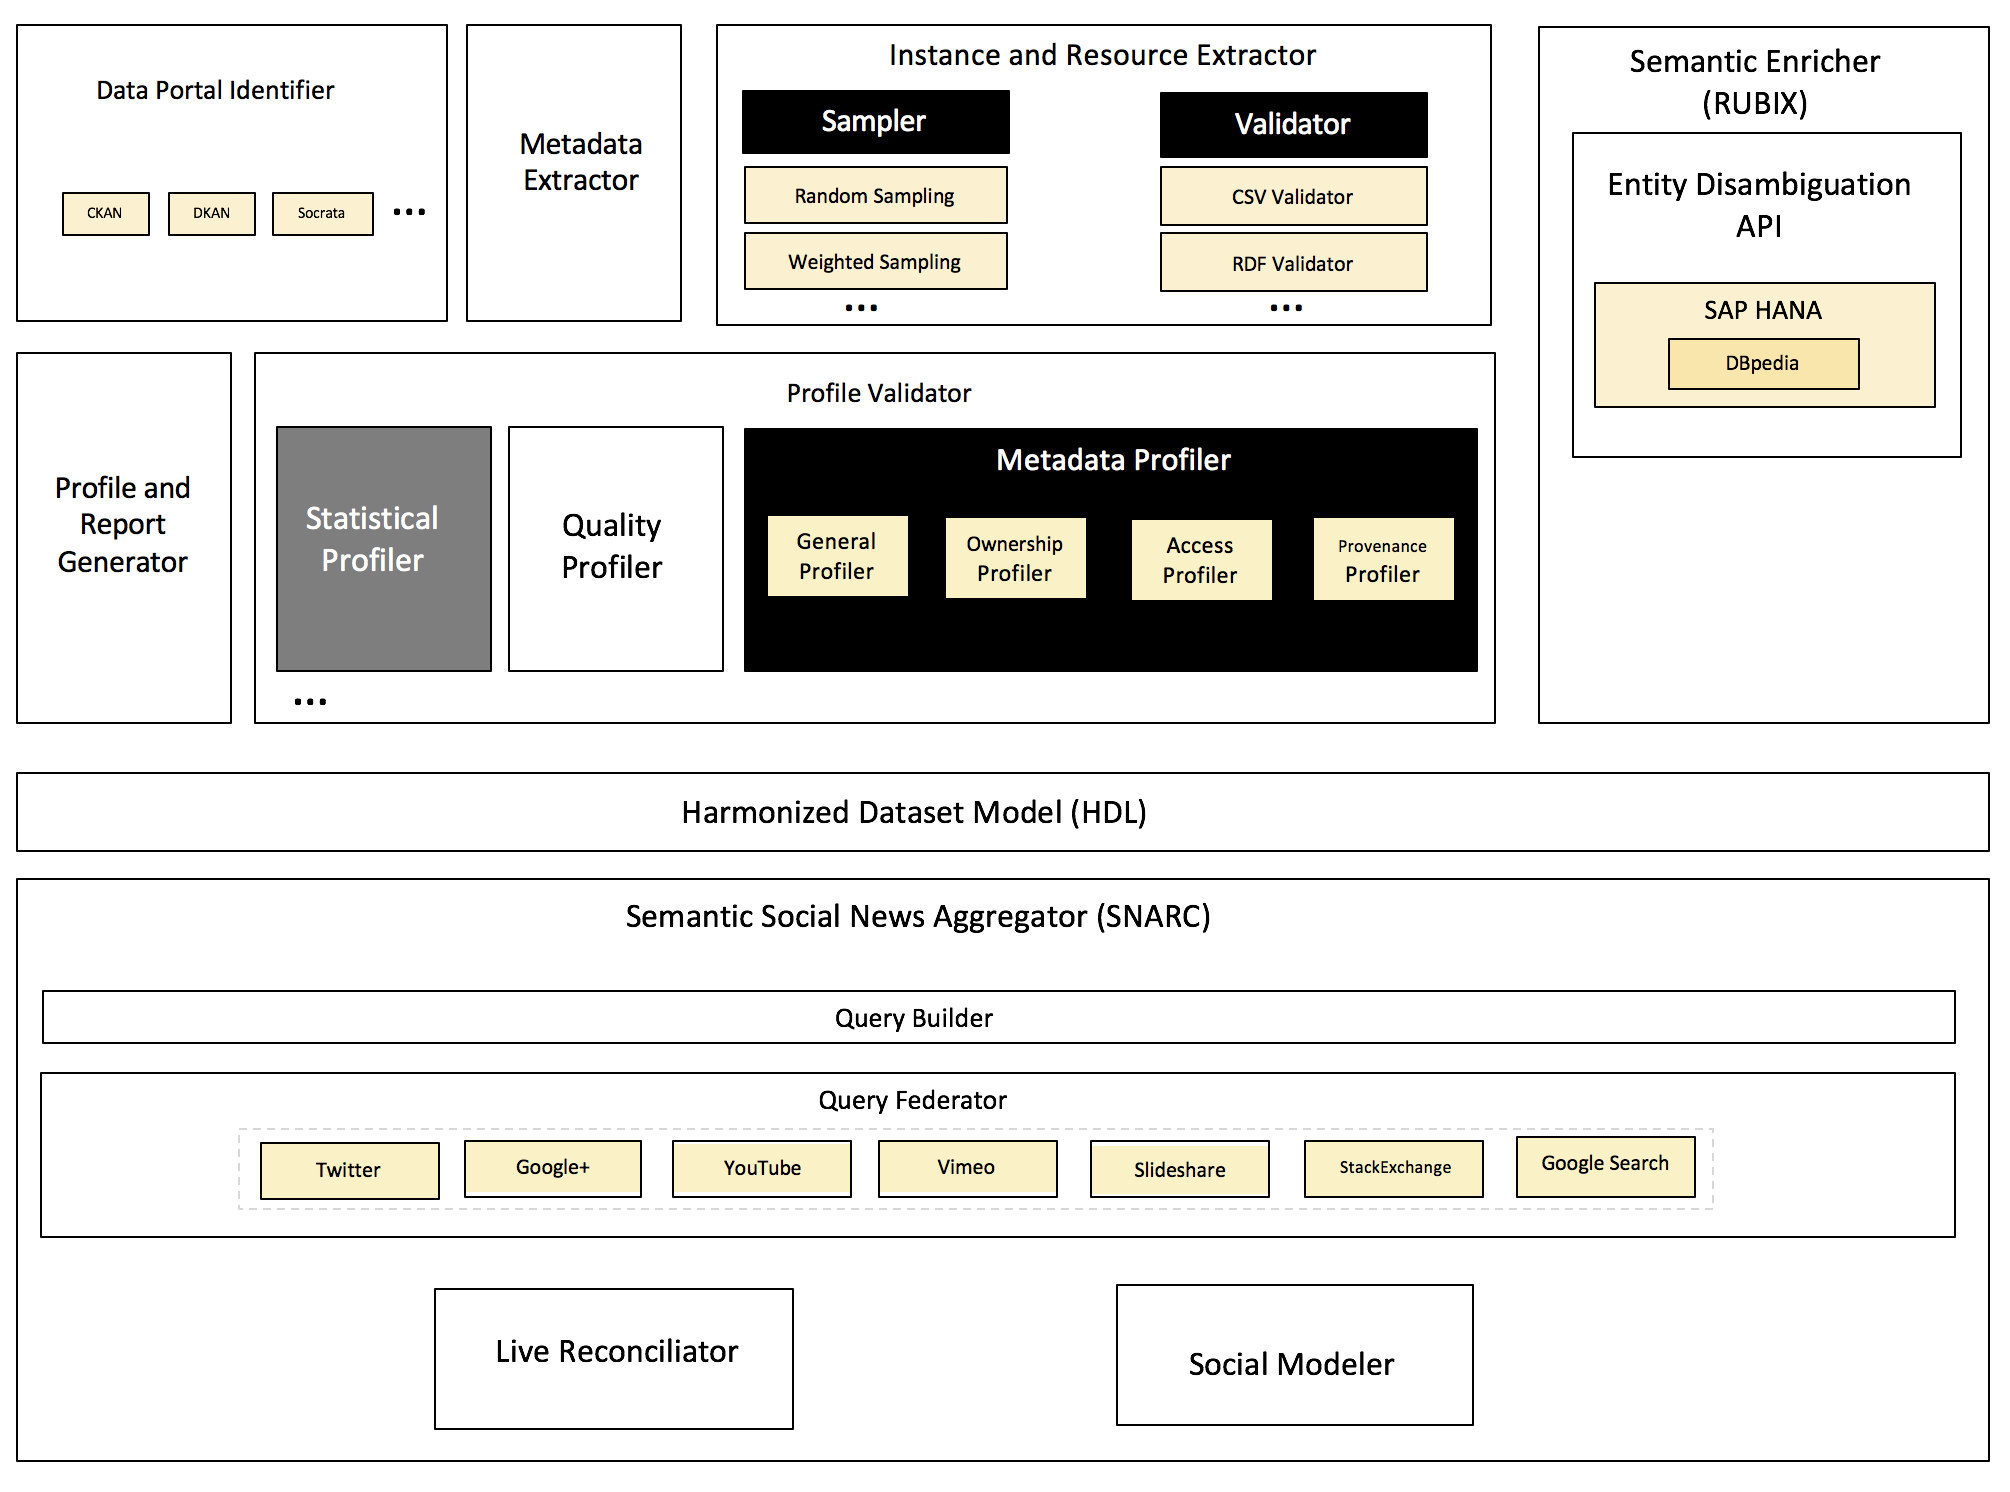
\includegraphics[scale=0.4]{architecutre_diagram.png}
	\caption{Sch\'{e}ma de l'architecture des donn\'{e}es pour permettre l'acces en libre-service}
	\label{fig:architecutre_diagram_summary_french}
\end{figure}
\end{adjustwidth}

\subsection{Contributions sur la Maintenance et D\'{e}couverte des Donn\'{e}es}

En ce qui concerne cet aspect de notre recherche, nous avons accompli les tâches suivantes :
\begin{itemize}
\item Nous avons \'{e}tudi\'{e}s les diff\'{e}rents mod\`{e}les et vocabulaires qui d\'{e}crivent des ensembles de donn\'{e}es sur le web. Alors que l'utilisation d'un vocabulaire ou d'un mod\`{e}le commun est la cl\'{e} dans la communication, nous avons identifi\'{e} le besoin d'un mod\`{e}le de m\'{e}tadonn\'{e}es harmonis\'{e} contenant suffisamment d'informations afin que les consommateurs puissent facilement comprendre et analyser les donn\'{e}es. Premi\`{e}rement, nous avons mis en place un ensemble de correspondances entre chacune des propri\'{e}t\'{e}s des mod\`{e}les \'{e}tudi\'{e}s. Ceci a conduit \`{a} la conception de HDL, un mod\`{e}le de donn\'{e}es harmonis\'{e}e, qui prend le meilleur sur les mod\`{e}les \'{e}tudi\'{e}s et les \'{e}tend pour assurer une couverture compl\`{e}te de m\'{e}tadonn\'{e}es lors de la d\'{e}couverte, exploration et la r\'{e}utilisation des donn\'{e}es.
\item Nous avons analys\'{e} l'ensemble des outils de profilage de source de donn\'{e}es et d\'{e}couvert de s\'{e}rieuses lacunes. En cons\'{e}quence, nous avons propos\'{e} Roomba, un outil \'{e}volutif pour automatiquement extraire, valider, cr\'{e}er et g\'{e}n\'{e}rer des profils de m\'{e}tadonn\'{e}es d\'{e}crivant les donn\'{e}es li\'{e}es. Roomba applique plusieurs techniques afin de v\'{e}rifier la validit\'{e} des m\'{e}tadonn\'{e}es fournies et pour g\'{e}n\'{e}rer des informations descriptives et statistiques sur un ensemble de donn\'{e}es particulier ou alors pour un portail de donn\'{e}es complet.
\end{itemize}

\subsection{Contributions sur la Qualit\'{e} des Donn\'{e}es}
Concernant nos contributions sur l'\'{e}valuation de la qualit\'{e} des donn\'{e}es li\'{e}es (Linked Data), nous avons accompli les tâches suivantes :
\begin{itemize}
\item Nous avons propos\'{e} un cadre d'\'{e}valuation de la qualit\'{e} des donn\'{e}es li\'{e}es en se concentrant sur des mesures objectives. Nous avons identifi\'{e} un total de 64 indicateurs de qualit\'{e} qui ont \'{e}t\'{e} r\'{e}partis en quatre cat\'{e}gories principales (entit\'{e}, source de donn\'{e}es, liens, mod\`{e}les) correspondant aux principes de la publication des ``Linked Data''.
\item Sur l'\'{e}tude des diff\'{e}rents outils de qualit\'{e} de donn\'{e}es, nous avons remarqu\'{e} un manque d'automatisation pour v\'{e}rifier les mesures propos\'{e}es dans notre approche. En cons\'{e}quence, nous avons \'{e}tendu Roomba pour effectuer une s\'{e}rie de contr\^{o}les de qualit\'{e} des donn\'{e}es sur les ensembles de donn\'{e}es li\'{e}s. Notre extension couvre la plupart des indicateurs de qualit\'{e} propos\'{e}s avec un accent sur l'exhaustivit\'{e}, l'exactitude, la provenance et les licences utilis\'{e}es.
\end{itemize}

\subsection{Contributions sur l'int\'{e}gration et l'am\'{e}lioration des Donn\'{e}es}

En ce qui concerne cet aspect de notre recherche, nous avons accompli les tâches suivantes :
\begin{itemize}
\item Nous avons cr\'{e}\'{e} un framework appel\'{e} RUBIX qui permet d'utiliser des donn\'{e}es provenant de sources peu structur\'{e}es et priv\'{e}es \`{a} des sources publiques et clairement structur\'{e}es. Le framework exploite des bases de connaissances de r\'{e}f\'{e}rence pour annoter des donn\'{e}es avec des concepts s\'{e}mantiques (m\'{e}tadonn\'{e}es). Un des avantages de ces m\'{e}tadonn\'{e}es est d'am\'{e}liorer le processus d'identification de donn\'{e}es similaire \`{a} partir de sources h\'{e}t\'{e}rog\`{e}nes au sein d'une entreprise.
\item Les m\'{e}tadonn\'{e}es attach\'{e}es par RUBIX peuvent encore \^{e}tre utilis\'{e}e pour enrichir les ensembles de donn\'{e}es existants. Toutefois, les concepts sont souvent repr\'{e}sent\'{e}s avec un grand ensemble de propri\'{e}t\'{e}s. Pour recommander les plus ``importantes'' propri\'{e}t\'{e}s d'un concept, nous avons analys\'{e} les choix faits par Google avec de la retro-ing\'{e}nierie lors de la cr\'{e}ation de graphiques et pr\'{e}sent\'{e}s ces choix en utilisant le vocabulaire de Fresnel, de sorte que toute application peut lire ce vocabulaire pour d\'{e}cider les propri\'{e}t\'{e}s int\'{e}ressantes d'une entit\'{e}.
\item L'agr\'{e}gation des informations des nouvelles sociales n'est pas une tâche facile. Nous fournissons une interface de programmation (API) qui permet l'agr\'{e}gation des r\'{e}seaux sociaux appel\'{e} SNARC. Nous avons conçu un exemple d'application web tirant parti des capacit\'{e}s de SNARC pour permettre aux utilisateurs de d\'{e}couvrir instantan\'{e}ment les nouvelles pertinentes des r\'{e}seaux sociaux.
\end{itemize}

%%%%%%%%%%%%%%%%%%%%%%%%%
%%% Towards A Complete Dataset Profile %%%
%%%%%%%%%%%%%%%%%%%%%%%%%
\let\cleardoublepage\clearpage\let\cleardoublepage\clearpage
\section{Vers un Profil de Donn\'{e}es Complet}

%%%%%%%%%%%%%%%%%%%%%%%%%
%%% Dataset Profiles and Models %%%
%%%%%%%%%%%%%%%%%%%%%%%%%

\subsection{Profils et Mod\`{e}les d'ensembles de Donn\'{e}es}

L'utilit\'{e} des donn\'{e}es ouvertes (Open Data) se reconnait \`{a} partir du moment o\`{u} on en a besoin. Les fournisseurs de donn\'{e}es se doivent de fournir des donn\'{e}es faciles \`{a} retrouver. Les portails de donn\'{e}es sont sp\'{e}cifiquement conçus \`{a} cet effet. Ils rendent facile pour les individus et les organisations le stockage, la publication et la d\'{e}couverte des ensembles de donn\'{e}es.

Les portails de donn\'{e}es (ou des catalogues de donn\'{e}es) sont les points d'entr\'{e}e pour d\'{e}couvrir les jeux de donn\'{e}es publi\'{e}s. Ils sont les garants des jeux de donn\'{e}es et de m\'{e}tadonn\'{e}es qu'ils h\'{e}bergent, tout en fournissant un ensemble de services de d\'{e}couverte et d'int\'{e}gration compl\'{e}mentaires.

Les portails de donn\'{e}es peuvent \^{e}tre public comme \texttt{Datahub.io} et \texttt{publicdata.eu} ou priv\'{e} comme \texttt{quandl.com} et \texttt{enigma.io}. Les portails priv\'{e}s exploitent des donn\'{e}es consolid\'{e}es manuellement provenant de diverses sources et les exposent \`{a} des utilisateurs soit librement, soit par le biais de licences. De la m\^{e}me mani\`{e}re, dans certains portails de donn\'{e}es publiques, les administrateurs examinent manuellement les informations des bases de donn\'{e}es, les valide, les corrige et leur attache des informations de m\'{e}tadonn\'{e}es appropri\'{e}. Cette information est principalement sous la forme de tag pr\'{e}d\'{e}finis telles que \textit{m\'{e}dias, g\'{e}ographie, sciences de la vie} pour des raisons d'organisation et de r\'{e}partition.

Il existe plusieurs syst\`{e}mes de gestion de donn\'{e}es (DMS) qui agr\'{e}mente les portails publics. CKAN\footnote{\url{http://ckan.org}} est le leader open-source de portail de donn\'{e}es, propulsant des sites web comme DataHub, les donn\'{e}es publiques de l'Europe et des donn\'{e}es ouvertes du gouvernement am\'{e}ricain. Model\'{e} sur CKAN, DKAN\footnote{\url{http://nucivic.com/dkan/}} est une distribution Drupal qui est utilis\'{e}e dans diff\'{e}rents portails de donn\'{e}es publiques. En plus de ces portails de donn\'{e}es, il y a un ensemble d'outils qui permettent d'exposer directement les donn\'{e}es via des API RESTful, tel que \texttt{thedatatank.com}.

Un ensemble de donn\'{e}es repr\'{e}sentant un mod\`{e}le de m\'{e}tadonn\'{e}es doit contenir suffisamment d'informations afin que les consommateurs puissent facilement comprendre et traiter les donn\'{e}es qui sont d\'{e}crites. Apr\`{e}s avoir analys\'{e} les mod\`{e}les d'ensembles de donn\'{e}es les plus importants, nous d\'{e}terminons qu'un ensemble de donn\'{e}es contient quatre sections principales :
\begin{itemize}
	\item \textbf{Ressources}:Les donn\'{e}es brutes peuvent \^{e}tre t\'{e}l\'{e}charg\'{e} ou accessible directement via des requ\^{e}tes. Les ressources peuvent \^{e}tre fournies dans diff\'{e}rents formats tels que JSON, XML ou RDF.
	\item \textbf{Tags}:Une description plus pouss\'{e}e \`{a} propos du contenu et de la structure du jeu de donn\'{e}es. Cela peut aller de la repr\'{e}sentation textuelle simple \`{a} des termes s\'{e}mantiques riches. Les tags sont la base de pour d\'{e}finir une recherche et d\'{e}couverte de donn\'{e}es.
	\item \textbf{Groupes}:Les groupes agissent comme des unit\'{e}s organisationnelles qui partagent une s\'{e}mantique commune. Ils peuvent \^{e}tre consid\'{e}r\'{e}s comme un ensemble de jeu de donn\'{e}es bas\'{e}s sur des cat\'{e}gories ou des th\`{e}mes communs.
	\item \textbf{Organisations}:Les organisations sont une autre façon d'organiser les ensembles de donn\'{e}es. Cependant, ils diff\`{e}rent des groupes car ils ne partagent pas des propri\'{e}t\'{e}s ou une s\'{e}mantique commune, mais reposent uniquement sur l'association de l'ensemble de donn\'{e}es \`{a} un tiers d'administration sp\'{e}cifique.
\end{itemize}

Apr\`{e}s une \'{e}tude pouss\'{e}e des diff\'{e}rents mod\`{e}les de donn\'{e}es, nous avons regroup\'{e} les informations de m\'{e}tadonn\'{e}es en huit types principaux. Chaque section d\'{e}crite ci-dessus doit contenir un ou plusieurs de ces types. Par exemple, les ressources ont les types suivants : g\'{e}n\'{e}ral, acc\`{e}s, droits, provenance alors que les tags sont : g\'{e}n\'{e}ral et provenance seulement. Les huit types d'information sont :
\begin{itemize}
	\item \textbf{Informations G\'{e}n\'{e}rales} :L'information de base \`{a} propos de l'ensemble de donn\'{e}es (i.e, titre, description, ID). Le vocabulaire le plus couramment utilis\'{e} pour d\'{e}crire cette information est Dublin Core\footnote{\url{http://dublincore.org/documents/dcmi-terms/}}.
	\item \textbf{Informations d'Acc\`{e}s} : Informations sur l'acc\`{e}s et l'utilisation de l'ensemble de donn\'{e}es (par exemple, l'URL, le titre de la licence et son URL associ\'{e}e). En plus des propri\'{e}t\'{e}s d\'{e}crites dans les mod\`{e}les ci-dessus, il y a plusieurs vocabulaires sp\'{e}cialement conçus pour d\'{e}crire les droits d'acc\`{e}s aux donn\'{e}es, par exemple, Linked Data Rights\footnote{\url{http://oeg-dev.dia.fi.upm.es/licensius/static/ldr/}}, l'Open Digital Rights Language (ODRL)\footnote{\url{http://www.w3.org/ns/odrl/2/}}.
	\item \textbf{Informations de Droits} : Informations de r\'{e}f\'{e}rence sur l'ensemble de donn\'{e}es (par exemple, auteur, responsable et organisation). Les vocabulaires communs utilis\'{e}s pour exposer des informations de propri\'{e}t\'{e} sont Friend-of-Friend (FOAF)\footnote{\url{http://xmlns.com/foaf/spec/}} pour les personnes et les relations, vCard~\cite{Iannella:W3C:14} pour les personnes et les organisations et l'Organization ontology~\cite{Reynolds:W3C:14} conçu sp\'{e}cifiquement pour d\'{e}crire les structures organisationnelles.
	\item \textbf{Informations de Provenance} : Informations temporelle et historique sur la cr\'{e}ation et mise \`{a} jour de l'ensemble de donn\'{e}es, en plus des informations sur les versions (par exemple, la donn\'{e}es de cr\'{e}ation, les donn\'{e}es sur la mise \`{a} jour des m\'{e}tadonn\'{e}es, derni\`{e}re version). Le renseignement de la provenance de l'information varie \`{a} travers le mod\`{e}le \'{e}tudi\'{e}. Cependant, son importance a conduit \`{a} l'\'{e}laboration de divers vocabulaires sp\'{e}ciaux comme l'Open Provenance Model\footnote{\url{http://open-biomed.sourceforge.net/opmv/}} et le PROV-O~\cite{Lebo:W3C:13}. DataID~\cite{Brummer::ICSS:14} est un effort pour fournir des m\'{e}tadonn\'{e}es s\'{e}mantiquement riche en mettant l'accent sur la source de l'information, la licence associ\'{e}e et les informations d'acc\`{e}s.
	\item \textbf{L'information G\'{e}ospatiale} : Information refl\'{e}tant la couverture g\'{e}ographique de l'ensemble de donn\'{e}es repr\'{e}sent\'{e} avec des coordonn\'{e}es ou des polygones. Il existe plusieurs mod\`{e}les et extensions sp\'{e}cifiquement conçus pour exprimer des informations g\'{e}ographiques suppl\'{e}mentaires. La directive ``Infrastructure for Spatial Information in the European Community'' (INSPIRE)\footnote{\url{http://inspire.ec.europa.eu/}} vise \`{a} \'{e}tablir une infrastructure d'information spatiale. Des connections ont \'{e}t\'{e} \'{e}tablis entre l'EDSC-AP et les m\'{e}tadonn\'{e}es de INSPIRE. CKAN fournit ainsi une extension spatiale\footnote{\url{https://github.com/ckan/ckanext-spatial}} afin d'ajouter des informations g\'{e}ospatiales. Il permet d'importer des m\'{e}tadonn\'{e}es g\'{e}ospatiales \`{a} partir d'autres ressources et fonctionne avec diverses normes (par exemple, ISO 19139) et formats (par exemple, GeoJSON).
	\item \textbf{Information temporelle} : Information refl\'{e}tant la couverture temporelle de l'ensemble de donn\'{e}es (par exemple, de date \`{a} date). Il y a eu un travail remarquable sur l'extension CKAN pour inclure des informations temporelles. \texttt{govdata.de} est un portail Open Data en Allemagne qui \'{e}tend le mod\`{e}le de donn\'{e}es CKAN avec des informations comme \texttt{temporal\_granularity}, \texttt{temporal\_coverage\_to} and \texttt{temporal\_granularity\_from}.
	\item \textbf{Informations statistiques} : des informations statistiques sur les types de donn\'{e}es et leur redondance dans les ensembles de donn\'{e}es (par exemple, la distribution des propri\'{e}t\'{e}s, nombre d'entit\'{e}s et triplets RDF). Cette information est particuli\`{e}rement utile pour explorer un ensemble de donn\'{e}es, car il donne un aperçu d\'{e}taill\'{e} sur les donn\'{e}es brutes. VoID est le seul mod\`{e}le qui fournit des informations statistiques sur un ensemble de donn\'{e}es. VoID d\'{e}finit des propri\'{e}t\'{e}s pour exprimer diff\'{e}rentes caract\'{e}ristiques statistiques sur un ensemble de donn\'{e}es comme le nombre total de triplets, le nombre total d'entit\'{e}s, le nombre total de classes distinctes, etc. Cependant, il existe d'autres vocabulaires tels que SCOVO~\cite{Hausenblas:ESWC:09} qui peut mod\'{e}liser et publier des donn\'{e}es statistiques sur les ensembles de donn\'{e}es.
	\item \textbf{Information de qualit\'{e}}:L'information qui indique la qualit\'{e} de l'ensemble de donn\'{e}es sur les niveaux de m\'{e}tadonn\'{e}es. En plus de cela, un ensemble de donn\'{e}es devrait inclure une \'{e}chelle qui mesure le respect des normes de publication des standards des Linked Data~\cite{Berners-Lee:W3C:06}. Une information de qualit\'{e} est seulement exprim\'{e}e dans les m\'{e}tadonn\'{e}es de POD. Cependant, \texttt{govdata.de} \'{e}tend le mod\`{e}le de CKAN pour y inclure un champ \texttt{ratings\_average}. En outre, il existe plusieurs autres vocabulaires comme daQ~\cite{Debattista:WWW:14} qui peuvent \^{e}tre utilis\'{e}s pour exprimer la qualit\'{e} des ensembles de donn\'{e}es. Le RDF Review Vocabulary\footnote{\url{http://vocab.org/review/}} peut \'{e}galement \^{e}tre utilis\'{e} pour exprimer les commentaires et \'{e}valuations sur l'ensemble de donn\'{e}es et de ses ressources.
\end{itemize}

Alors que l'utilisation d'un vocabulaire ou d'un mod\`{e}le commun est la cl\'{e} de la communication, nous avons identifi\'{e} le besoin d'un mod\`{e}le harmonis\'{e}e de m\'{e}tadonn\'{e}es contenant suffisamment d'informations pour que les consommateurs puissent facilement comprendre et appr\'{e}hender les donn\'{e}es. Pour cr\'{e}er les correspondances entre les diff\'{e}rents mod\`{e}les, nous avons proc\'{e}d\'{e} en plusieurs \'{e}tapes :
\begin{itemize}
	\item Examiner tous les mod\`{e}les, les sp\'{e}cifications des vocabulaires et les documentations.
	\item Examiner les ensembles de donn\'{e}es existantes en utilisant ces mod\`{e}les et vocabulaires. Data Portal\footnote{\url{http://dataportals.org}} fournit une liste compl\`{e}te des portails ouverts de donn\'{e}es du monde entier. Ca a \'{e}t\'{e} notre point de d\'{e}part pour trouver les portails utilisant CKAN ou DKAN comme syst\`{e}me de gestion de donn\'{e}es (DMS). Socrata, par exemple, maintient une liste des portails Open Data utilisant leur logiciel sur leur page d'accueil comme \url{http://pencolorado.org} et \url{http://data.maryland.gov}.
	\item Examiner le code source de certains portails. Ce fut particuli\`{e}rement le cas pour Socrata, car leur API renvoie les donn\'{e}es brutes s\'{e}rialis\'{e}es en JSON plut\^{o}t que les m\'{e}tadonn\'{e}es de l'ensemble de donn\'{e}es. En cons\'{e}quence, nous avons dû \'{e}tudier le code source de l'API Socrata Open Data (SODA)\footnote{\url{https://github.com/socrata/soda-java/tree/master/src/main/java/com/socrata/model}} pour r\'{e}cup\'{e}rer les diff\'{e}rentes classes et interfaces.
\end{itemize}

De notre \'{e}tude, nous avons constat\'{e} qu'une bonne int\'{e}gration des donn\'{e}es de l'Open Data dans les entreprises n\'{e}cessite une am\'{e}lioration des ensembles de donn\'{e}es pour inclure les informations suivantes :
\begin{itemize}
	\item\textbf{informations d'acc\`{e}s} : un ensemble de donn\'{e}es est inutile s'il ne contient pas de m\'{e}canismes pour r\'{e}cup\'{e}rer les donn\'{e}es, ou de point central pour effectuer des requ\^{e}tes.
	\item\textbf{informations de licence} : les entreprises sont toujours pr\'{e}occup\'{e}es par les implications juridiques de l'utilisation du contenu externe. En cons\'{e}quence, les ensembles de donn\'{e}es devraient inclure \`{a} la fois des informations compr\'{e}hensible par les individus mais aussi automatiquement par des logiciels, comme les informations de permissions, droits d'auteur et attributions.
	\item\textbf{information de provenance} : en fonction de la licence du jeu de donn\'{e}es, les donn\'{e}es pourraient ne pas \^{e}tre l\'{e}galement utilisable s'il n'y a pas d'information d\'{e}crivant les auteurs et les modifications effectu\'{e}es. Les mod\`{e}les actuels ne respectent pas ces contraintes, limitant de fait l'utilisation de nombreux ensembles de donn\'{e}es.
\end{itemize}

Nous avons identifi\'{e} quatre sections principales qui devraient \^{e}tre incluses dans le mod\`{e}le : les ressources, les groupes, les tags et les organisations. En outre, nous avons d\'{e}fini huit types pour classifier l'information. Notre principale contribution est la d\'{e}finition de correspondances entre chacune des propri\'{e}t\'{e}s de ces mod\`{e}les. Ceci a conduit \`{a} la conception de HDL, un mod\`{e}le de donn\'{e}es harmonis\'{e}e, qui prend le meilleur des mod\`{e}les pour assurer une couverture compl\`{e}te de m\'{e}tadonn\'{e}es facilitant la d\'{e}couverte, exploration et la r\'{e}utilisation de donn\'{e}es.

%%%%%%%%%%%%%%%%%%%%%%%%%
%%% Dataset Profiles Generation and Validation %%%
%%%%%%%%%%%%%%%%%%%%%%%%%
\subsection{G\'{e}n\'{e}ration et Validation de Profils de Donn\'{e}es}

La nature h\'{e}t\'{e}rog\`{e}ne des sources de donn\'{e}es influe directement sur la qualit\'{e} des donn\'{e}es, car elles contiennent souvent des incoh\'{e}rences ainsi que des m\'{e}tadonn\'{e}es incompl\`{e}tes et mal interpr\'{e}t\'{e}es. En outre, la variation significative de la taille, de formats et la fraîcheur des donn\'{e}es rend plus difficile la recherche d'ensemble de donn\'{e}es utiles sans connaissance pr\'{e}alable. On remarque tr\`{e}s bien ce point dans le cloud de Linked Open Data o\`{u} quelques ensembles de donn\'{e}es tels que DBPedia~\cite{Bizer:WebSemJorunal:09}, Freebase~\cite{Bollacker:SIGMOD:08} et YAGO~\cite{Suchanek::WWW:07} sont favoris\'{e}s par rapport \`{a} des ensembles de donn\'{e}es moins populaires, mais qui sont plus adaptes avec un domaine sp\'{e}cifique pour les tâches \`{a} accomplir. Par exemple, pour construire des syst\`{e}mes de recommandation \`{a} partir d'une biblioth\`{e}que num\'{e}rique universitaire dans le cloud LOD, les ensembles de donn\'{e}es populaires comme le Semantic Web Dog Food\footnote{\url{http://datahub.io/dataset/semantic-web -Dog-alimentaire}}, DBLP\footnote{\url{http://datahub.io/dataset/dblp}} ou Yovisto\footnote{\url{http://datahub.io/dataset/yovisto}} peuvent \^{e}tre favoris\'{e}s par rapport \`{a} des ensembles de donn\'{e}es moins connus, mais plus sp\'{e}cifiques comme VIAF\footnote{\url{http://datahub.io/dataset/viaf}} qui relie les fichiers d'autorit\'{e} de 20 biblioth\`{e}ques nationales, une liste des sujets des titres des biblioth\`{e}ques publiques en Espagne\footnote{\url{http://datahub.io/dataset/lista-encabezamientos-materia}} ou les recherche de th\`{e}se françaises\footnote{\url{http://datahub.io/dataset/thesesfr}}.

Les utilisateurs explorent des ensembles de donn\'{e}es dans des portails en se basant sur les m\'{e}tadonn\'{e}es propos\'{e}es par le propri\'{e}taire de l'ensemble de donn\'{e}es ou l'administrateur du portail de donn\'{e}es. Cette information est principalement disponible sous la forme de tags pr\'{e}d\'{e}finis tels que \textit{m\'{e}dias, g\'{e}ographie, sciences de la vie} qui sont utilis\'{e}s \`{a} des fins d'organisation et de regroupement. Cependant, la diversit\'{e} croissante de ces ensembles de donn\'{e}es rend plus difficile le classement dans un nombre restreint de tags, qui sont subjectivement attribu\'{e}s sans jamais capturer l'essence et l'\'{e}tendue de l'ensemble de donn\'{e}es~\cite {Lalithsena:WI:13}. En outre, l'augmentation du nombre d'ensembles de donn\'{e}es disponible rend l'analyse manuelle et la conservation des m\'{e}tadonn\'{e}es insoutenable, m\^{e}me quand cette tache est confi\'{e}e \`{a} des communaut\'{e}s.

Roomba est un outil que nous proposons pour adresser les probl\'{e}matique de validation et de g\'{e}n\'{e}ration automatique de profils d'ensemble de donn\'{e}es descriptifs. C'est un framework extensible qui consiste en une ex\'{e}cution structur\'{e}e combinant des techniques d'identification de portails de donn\'{e}es, de r\'{e}cup\'{e}ration de jeux de donn\'{e}es, et d'un ensemble de modules assemblable en combinant plusieurs tâches. Le framework valide les m\'{e}tadonn\'{e}es attach\'{e}es \`{a} l'ensemble de donn\'{e}es en les confrontant \`{a} un ensemble de donn\'{e}es agr\'{e}g\'{e}es. Les champs des m\'{e}tadonn\'{e}es sont automatiquement corrig\'{e}s quand c'est possible (par exemple, ajout de l'URL d'une licence manquante). En outre, un rapport d\'{e}crivant tous les probl\`{e}mes qui ne peuvent \^{e}tre automatiquement r\'{e}solus est cr\'{e}\'{e} pour \^{e}tre envoy\'{e} par courriel au responsable de l'ensemble de donn\'{e}es. Il existe diff\'{e}rents outils de profilage statistiques pour les donn\'{e}es relationnelles et les Linked Data. L'architecture du framework permet de facilement int\'{e}grer ces outils pour approfondir le profilage. Cependant, dans cette section, nous nous concentrons sur le profilage des m\'{e}tadonn\'{e}es d'un jeu de donn\'{e}es en ignorant les tâches de profilage statistique. Nous validons notre framework \`{a} l'aide d'un ensemble de profils cr\'{e}\'{e}s manuellement et v\'{e}rifions manuellement la pr\'{e}cision des r\'{e}sultats par rapport \`{a} ceux fournis par des portails bases sur CKAN.

Roomba est propos\'{e} comme un outil en ligne de commande (CLI) en utilisant Node.js et est disponible sur la plateforme GitHub\footnote{\url{https://github.com/ahmadassaf/opendata-checker/tree/master/test}}. Roomba permet aux administrateurs de portail de donn\'{e}es comme \textbf{Dan} de:

\begin{itemize}
	\item R\'{e}cup\'{e}rer des informations sur le syst\`{e}me de gestion des donn\'{e}es du portail
	\item R\'{e}cup\'{e}rer toutes les informations sur les ensembles de donn\'{e}es \`{a} partir d'un portail
	\item R\'{e}cup\'{e}rer toutes les informations de groupe \`{a} partir d'un portail de donn\'{e}es
	\item Parcourir, chercher et mettre en cache des jeux de donn\'{e}es (un ensemble de donn\'{e}es sp\'{e}cifiques, des ensembles de donn\'{e}es d'un groupe, des ensembles de donn\'{e}es sur l'ensemble du portail)
	\item Ex\'{e}cuter un programme d'agr\'{e}gation sur un groupe sp\'{e}cifique ou sur le portail entier
	\item Analyser un ensemble de donn\'{e}es sp\'{e}cifique, un ensemble du groupe ou le portail entier
\end{itemize}

La Figure~\ref{fig:architecutre_diagram_summary_french} montre les principales \'{e}tapes :

\begin{itemize}
	\item \textbf{Identification de syst\`{e}me de gestion de donn\'{e}es}: L'identificateur de portail repose sur plusieurs techniques de r\'{e}cup\'{e}ration lors de la phase d'identification. Elle comprend une combinaison d'inspection de l'URL, une revue des m\'{e}tadonn\'{e}es, et une inspection du Document Object Model (DOM).
	\item \textbf{Extraction des m\'{e}tadonn\'{e}es} : Apr\`{e}s avoir identifi\'{e} la plateforme sous-jacente du portail, le module d'extraction des m\'{e}tadonn\'{e}es envoie des requ\^{e}tes a l'API afin de r\'{e}cup\'{e}rer l’ensemble des m\'{e}tadonn\'{e}es puis les entrepose dans un syst\`{e}me de cache. Selon la plateforme utilis\'{e}e, l'extracteur peut lancer des taches sp\'{e}cifiques. Par exemple, dans les portails bas\'{e}s CKAN, l'extracteur est capable de parcourir et extraire les m\'{e}tadonn\'{e}es d'un ensemble de donn\'{e}es sp\'{e}cifique, tous les ensembles de donn\'{e}es d'un groupe donn\'{e} (par exemple, LOD cloud) ou tous les jeux de donn\'{e}es du portail.
	\item \textbf{Extraction des ressources et des instances}: Des m\'{e}tadonn\'{e}es extraites, le module d'extraction de ressources est capable d'identifier toutes les ressources associ\'{e}es a un jeu de donn\'{e}es. Ils peuvent avoir diff\'{e}rents types comme une instance SPARQL, API, fichier, visualisation, etc. Cependant, avant d'extraire l'int\'{e}gralit\'{e} des ressources d'un serveur, et consid\'{e}rant que l'ensemble des donn\'{e}es contient potentiellement de grandes quantit\'{e}s de ressources et que la puissance de calcul est limit\'{e}e pour certains serveur, un sous-module permet de r\'{e}cup\'{e}rer des \'{e}chantillons. Diff\'{e}rentes strat\'{e}gies \`{a} base d'\'{e}chantillons existent, et peuvent produire des r\'{e}sultats pr\'{e}cis, m\^{e}me avec des petits \'{e}chantillons d'environ 10\% des donn\'{e}es~\cite{Fetahu:ESWC:14}.
	\item \textbf{Validation du profil} : Le module de validation du profil (composant (iv)) identifie les informations manquantes et a la capacit\'{e} de les corriger automatiquement. Chaque ensemble de m\'{e}tadonn\'{e}es (g\'{e}n\'{e}ral, acc\`{e}s, possession et provenance) est valid\'{e} et corrig\'{e} automatiquement lorsque c'est possible. Chaque profilage v\'{e}rifie les champs de m\'{e}tadonn\'{e}es qu'il peut remplir. Le processus de validation v\'{e}rifie si chaque champ est d\'{e}fini et si la valeur attribu\'{e}e est valide.

	Il existe de nombreuses validations pour diff\'{e}rents domaines. Par exemple, les adresses \'{e}lectroniques et les URL doivent \^{e}tre valid\'{e}es pour garantir que la valeur entr\'{e}e est syntaxiquement correct. En plus de cela, pour les URL, le module de validation de profil \'{e}met une requ\^{e}te HTTP \texttt{HEAD} afin de v\'{e}rifier si cette URL est accessible. Le module utilise \'{e}galement les informations du \texttt{content-header} d'une r\'{e}ponse valide pour extraire, comparer et corriger certaines valeurs de m\'{e}tadonn\'{e}es des ressources comme \texttt{mimetype} et \texttt{size}.
	\item \textbf{G\'{e}n\'{e}ration du profil et de rapports} : Le processus de validation met en \'{e}vidence les informations manquantes et les pr\'{e}sente dans un rapport qui peut \^{e}tre automatiquement envoy\'{e} par email au mainteneur si son adresse est renseign\'{e}e dans les m\'{e}tadonn\'{e}es. En plus du rapport g\'{e}n\'{e}r\'{e}, les profils am\'{e}lior\'{e}s sont publi\'{e}s dans un format JSON en utilisant le mod\`{e}le de donn\'{e}es de CKAN et sont publiquement accessible\footnote{\url{https://github.com/ahmadassaf/opendata-checker/tree/master/results}}.
\end{itemize}

L'\'{e}tat actuel du rapport de cloud LOD~\cite{Schmachtenberg:ISWC:14} indique que le cloud LOD contient 1014 jeux de donn\'{e}es. Ils ont \'{e}t\'{e} r\'{e}colt\'{e}s via un robot de LDSpider~\cite{Isele:ISWC:10} \`{a} partir de 560 000 URI. Roomba r\'{e}cup\`{e}re les ensembles de donn\'{e}es h\'{e}berg\'{e}s dans les portails dont les m\'{e}tadonn\'{e}es sont pertinentes. Nous nous sommes appuy\'{e}s sur les informations fournies par l'API DataHub CKAN. En examinant les tags disponibles, nous avons trouv\'{e} deux groupes candidats. Le premier, marqu\'{e} avec ``lodcloud'', contient 259 ensembles de donn\'{e}es, tandis que le second, marqu\'{e} avec ``lod'' retourne seulement 75 ensembles de donn\'{e}es. Apr\`{e}s avoir examin\'{e} manuellement les deux listes, nous avons d\'{e}couvert que les jeux de donn\'{e}es group\'{e}s avec la balise ``lodcloud'' sont les bons car ils contenaient des m\'{e}tadonn\'{e}es plus r\'{e}cente et pr\'{e}cise. Pour aller plus loin, nous avons utilis\'{e} d'autres portails CKAN. Nous avons utilis\'{e} \texttt{dataportals.org}, qui contient une liste compl\`{e}te des portails Open Data \`{a} travers le monde. Nous avons choisi le portail de donn\'{e}es d'Amsterdam\footnote{\url{http://data.amsterdamopendata.nl/}}, car il est fr\'{e}quemment mis \`{a} jour et bien maintenu. Le portail a \'{e}t\'{e} command\'{e} en 2012 par le Amsterdam Economic Board Open Data Exchange (ODE), et couvre un large \'{e}ventail de domaines d'information (\'{e}nergie, \'{e}conomie, \'{e}ducation, d\'{e}veloppement urbain, etc.) sur Amsterdam.

Dans notre \'{e}valuation, nous nous sommes concentr\'{e}s sur deux aspects: i) \textit{la pertinence du profilage} qui \'{e}value manuellement la validit\'{e} des erreurs g\'{e}n\'{e}r\'{e}es dans le rapport, et ii) \textit{l'exhaustivit\'{e} du profilage} qui \'{e}value si les profils couvrent toutes les erreurs des m\'{e}tadonn\'{e}es des ensembles de donn\'{e}es.

Notre \'{e}valuation a montr\'{e} que Roomba propose une pertinence et une exhaustivit\'{e} accrue pour les propri\'{e}t\'{e}s examin\'{e}es. En cons\'{e}quence, nous avons ex\'{e}cut\'{e} Roomba sur le cloud LOD h\'{e}berg\'{e} dans le DataHub. Nous avons d\'{e}couvert que de nombreux ensemble de donn\'{e}es n\'{e}cessite des corrections. La plupart d'entre eux n'ont pas d'information d'acc\`{e}s et leurs ressources souffrent de faible disponibilit\'{e}. Ces deux mesures sont d'une grande importance pour les entreprises qui cherchent \`{a} int\'{e}grer et utiliser des donn\'{e}es externes. Nous avons d\'{e}couvert que l'information la plus erron\'{e}e est l'information de possession, puisque cette information est manquante ou ind\'{e}termin\'{e}e pour 41\% des ensembles de donn\'{e}es. Les ressources de jeux de donn\'{e}es ont les m\'{e}tadonn\'{e}es les plus pauvres : 64\% des m\'{e}tadonn\'{e}es g\'{e}n\'{e}rale, toutes les informations d'acc\`{e}s et 80\% de l'information sur la provenance des valeurs est manquante ou ind\'{e}termin\'{e}e. Nous avons \'{e}galement montr\'{e} que le processus de correction automatique peut effectivement am\'{e}liorer la qualit\'{e} de certaines informations. Nous croyons qu'il y a un besoin d'avoir un effort communautaire pour corriger manuellement les informations manquantes importantes comme des informations de possession (mainteneur, auteur, email de contact).

\subsection{\`{E}valuation Objective de la Qualit\'{e} des Donn\'{e}es Associ\'{e}es}

Nous entrons dans une \`{e}re o\`{u} l'ouverture devient le standard. Les gouvernements, les universit\'{e}s, les organisations et m\^{e}me les individus publient d'\'{e}normes quantit\'{e}s de donn\'{e}es ouvertes. Cette ouverture doit \^{e}tre accompagn\'{e}e d'un certain niveau de confiance, ainsi que des garanties sur la qualit\'{e} des donn\'{e}es. Le Linked Open Data est une mine d'or pour ceux qui essaient de tirer parti de sources de donn\'{e}es externes afin de produire des d\'{e}cisions plus \'{e}clair\'{e}es~\cite{Boyd:Article:11}. Cependant, l'h\'{e}t\'{e}rog\'{e}n\'{e}it\'{e} des sources impacte directement la qualit\'{e} des donn\'{e}es, car les sources contiennent souvent des informations mal interpr\'{e}t\'{e}es et incompl\`{e}tes.

La qualit\'{e} des donn\'{e}es est un domaine d'\'{e}tude minutieux avec de nombreux points d'\'{e}tudes et des frameworks pour en appr\'{e}cier ses dimensions~\cite{Kahn:ACM:02, Stvilia:ASIST:07, Wang:MIS:96}. Les principes de qualit\'{e} des donn\'{e}es reposent g\'{e}n\'{e}ralement sur de nombreux indicateurs subjectifs qui sont complexes \`{a} mesurer. La qualit\'{e} des donn\'{e}es est r\'{e}ellement appr\'{e}ci\'{e}e lors de son utilisation~\cite{Juran:McGraw:99}, donc est directement li\'{e}e \`{a} la capacit\'{e} de satisfaire les besoins des utilisateurs.

Les documents web qui sont par nature non structur\'{e}s et interconnectes n\'{e}cessitent des mesures de la qualit\'{e} et des techniques d'\'{e}valuation diff\'{e}rentes des ensembles de donn\'{e}es traditionnels. Par exemple, l'importance et la qualit\'{e} des documents web peuvent \^{e}tre subjectivement calcul\'{e}s par des algorithmes tels que le Page Rank~\cite{Page:TechReport:98}. Malgr\'{e} le fait que la qualit\'{e} des Linked Open Data est un sujet actuellement tr\`{e}s demand\'{e}, tr\`{e}s peu d'efforts sont en cours pour essayer de normaliser, suivre et formaliser les frameworks pour fournir des \'{e}valuations et des certificats qui aideront les consommateurs de donn\'{e}es dans leurs tâches d'int\'{e}gration.

L'\'{e}valuation de la qualit\'{e} des donn\'{e}es est un processus qui \'{e}value si un morceau de donn\'{e}e est conforme aux besoin dans un cas d'utilisation pr\'{e}cis~\cite{Bizer:WebSemantics:09}. La dimension de la qualit\'{e} des donn\'{e}es est li\'{e}e aux exigences qu'en ont les utilisateurs. Par exemple, DBpedia~\cite{Bizer:WebSemJorunal:09} et YAGO~\cite{Suchanek::WWW:07} sont des bases de connaissances contenant des donn\'{e}es extraites de sources structur\'{e}es et semi-structur\'{e}es. Ils sont utilis\'{e}s dans une vari\'{e}t\'{e} d'applications comme par exemple, des syst\`{e}mes d'annotation~\cite{Mendes:ICS:11}, des syst\`{e}mes d'exploration et de recherche~\cite{Marie:ICS:13} et des moteurs de recommandation~\cite{DiNoia:iSemantics:12}. Cependant, leurs donn\'{e}es ne sont pas int\'{e}gr\'{e}es dans des syst\`{e}mes critiques : applications m\'{e}dicales, applications a\'{e}ronautiques, etc. La qualit\'{e} des donn\'{e}es est jug\'{e}e insuffisante.

L'id\'{e}e de base \`{a} propos des Linked Data est qu'au plus elle est interconnect\'{e}e avec d'autres ensembles de donn\'{e}es, au plus son int\'{e}r\^{e}t grandit. Tim Berners-Lee a d\'{e}fini quatre grands principes pour la publication de donn\'{e}es qui peuvent assurer un certain niveau d'uniformit\'{e} qui refl\`{e}te directement leur utilisabilit\'{e}~\cite{Berners-Lee:W3C:06}:

\begin{itemize}
	\item Utiliser des URIs pour identifier les ressources.
	\item Utiliser des URIs HTTP pour acc\'{e}der de mani\`{e}re uniformis\'{e}e aux ressources.
	\item Fournir des repr\'{e}sentations en utilisant des langages et des protocoles standards (RDF, SPARQL).
	\item Inclure des liens pour permettre de d\'{e}couvrir de nouvelles ressources.
\end{itemize}

\noindent
Fort de ces principes, nous regroupons la qualit\'{e} des attributs en quatre cat\'{e}gories principales :

\begin{itemize}
	\item \textbf{Qualit\'{e} des entit\'{e}s}: indicateurs de qualit\'{e} qui mettent l'accent sur les donn\'{e}es au niveau de l'instance.
	\item \textbf{Qualit\'{e} de l'ensemble de donn\'{e}es}: indicateurs de qualit\'{e} au niveau de l'ensemble de donn\'{e}es.
	\item \textbf{Qualit\'{e} du mod\`{e}le s\'{e}mantique}: indicateurs de qualit\'{e} qui mettent l'accent sur les mod\`{e}les s\'{e}mantiques, les vocabulaires et ontologies.
	\item \textbf{Qualit\'{e} du processus de liaison}: indicateurs de qualit\'{e} qui mettent l'accent sur les liens entrants et sortants entre les ensembles de donn\'{e}es.
\end{itemize}

In~\cite{Assaf:DQMST:12}, les auteurs ont identifi\'{e} 24 attributs de qualit\'{e} de donn\'{e}es li\'{e}es diff\'{e}rentes. Ces attributs sont un m\'{e}lange de mesures objectives et subjectives qui ne peuvent pas \^{e}tre d\'{e}riv\'{e}es automatiquement. Dans cet article, nous affinons ces attributs dans un cadre condens\'{e} de 10 mesures objectives. \`{E}tant donn\'{e} que ces mesures sont plut\^{o}t abstraites, nous devrions compter sur les indicateurs de qualit\'{e} qui refl\`{e}tent la qualit\'{e} des donn\'{e}es~\cite{Flemming:Thesis:10} et les utiliser pour automatiser le calcul de la qualit\'{e} des ensembles de donn\'{e}es.

Les indicateurs de qualit\'{e} sont pond\'{e}r\'{e}s. Ces poids donnent la possibilit\'{e} de d\'{e}finir plusieurs degr\'{e}s d'importance. Par exemple, un ensemble de donn\'{e}es contenant les gens peuvent avoir plus d'une personne portant le m\^{e}me nom et il n'est donc pas toujours vrai que deux entit\'{e}s dans un jeu de donn\'{e}es ne devraient pas avoir le m\^{e}me label. En cons\'{e}quence, le poids de cet indicateur de qualit\'{e} sera mis \`{a} z\'{e}ro et ne n'affectera pas la note globale de qualit\'{e} pour la mesure de la coh\'{e}rence.

Les indicateurs ind\'{e}pendants pour la qualit\'{e} de l'entit\'{e} sont essentiellement subjectifs: par exemple, le niveau de d\'{e}tail sur les objets repr\'{e}sent\'{e}s, leur port\'{e}e etc. Les entit\'{e}s sont r\'{e}gies par le mod\`{e}le sous-jacent, et nous avons donc regroup\'{e} les indicateurs avec ceux de la qualit\'{e} de mod\'{e}lisation.

Les mesures et l'objectif des indicateurs de qualit\'{e} ont \'{e}t\'{e} recueillis en :

\begin{itemize}
	\item Transformant et consolidant les indicateurs de qualit\'{e} objectifs \`{a} partir d'une s\'{e}rie de questions~\cite{Assaf:DQMST:12}.
	\item Analysant et comparant les diff\'{e}rentes approches et outils sur la qualit\'{e} des donn\'{e}es.
	\item Examinant les propri\'{e}t\'{e}s des mod\`{e}les de Linked Data les plus courants \`{a} partir de l'\'{e}tude conduite dans~\cite{Assaf:PROFILES:15}.
\end{itemize}

Nous avons \'{e}tendu Roomba avec 7 sous-modules qui v\'{e}rifient les diff\'{e}rents indicateurs de qualit\'{e} de l'ensemble de donn\'{e}es. Certains indicateurs doivent \^{e}tre examin\'{e}s sur un ensemble fini. Puisque Roomba fonctionne sur des portails bases sur CKAN, nous avons construit notre extension de qualit\'{e} pour calculer les scores \`{a} partir du mod\`{e}le standard de CKAN.

Roomba couvre 82\% des indicateurs de qualit\'{e} objectifs propos\'{e}s. Sur la base de nos exp\'{e}rimentations avec Roomba sur le cloud LOD, nous avons d\'{e}couvert que la majorit\'{e} des ensembles de donn\'{e}es ont besoin de corrections. La plupart d'entre eux ne renseignent que tr\`{e}s mal la provenance, licence d'utilisation, et indicateurs de qualit\'{e}.

%%%%%%%%%%%%%%%%%%%%%%%%%
%%% Towards Enriched Enterprise Data %%%
%%%%%%%%%%%%%%%%%%%%%%%%%
\let\cleardoublepage\clearpage
\section{Vers des Donn\'{e}es d'entreprise Agr\'{e}ment\'{e}es}

\subsection{Int\'{e}gration des Donn\'{e}es dans l'entreprise}
Les entreprises effectuent traditionnellement des analyses et des rapports \`{a} partir de bases relationnelles. Les donn\'{e}es d'entreprise disponibles pour les d\'{e}cideurs \'{e}taient g\'{e}n\'{e}ralement la gestion des clients ou les donn\'{e}es de planification et ressources d'entreprise (ERP). Cependant, les informations en provenance des r\'{e}seaux sociaux, les blogs, les donn\'{e}es des capteurs, ou les donn\'{e}es publi\'{e}es par les gouvernements et organisations internationales sont de plus en plus accessibles~\cite{Boyd:Article:11}.

La qualit\'{e} et la quantit\'{e} de connaissance structur\'{e}e disponible rendent d\'{e}sormais possible pour les entreprises de parcourir cette \'{e}norme quantit\'{e} de donn\'{e}es publiques et de l'int\'{e}grer dans leurs syst\`{e}mes d'information. L'analyse de ces nouvelles donn\'{e}es dans le contexte des entreprises devrait leur apporter de nouvelles approche pour mieux appr\'{e}hender l'exploration et le ciblage de nouveaux marches~\cite{LaValle:MIT:11}.

Ces nouvelles sources distribu\'{e}es, cependant, posent des d\'{e}fis \'{e}normes. Elles ont diff\'{e}rents formats de fichiers, protocoles d'acc\`{e}s, ou encore diff\'{e}rents langages de requ\^{e}te. Elles poss\`{e}dent leur propre mod\`{e}le de donn\'{e}es avec diff\'{e}rentes façons de repr\'{e}senter et stocker les donn\'{e}es. Les donn\'{e}es \`{a} travers ces sources peuvent \^{e}tre dupliqu\'{e}es, incoh\'{e}rentes ou \^{e}tre s\'{e}mantiquement similaire et pourtant diff\'{e}rentes. L'int\'{e}gration et la d\'{e}finition d'une vue unifi\'{e}e pour ces structures de donn\'{e}es h\'{e}t\'{e}rog\`{e}nes et complexes n\'{e}cessitent donc des outils puissants pour cartographier et organiser les donn\'{e}es.

\`{E}tablir des bases de connaissances de donn\'{e}es dans l'entreprise peut faciliter la fourniture de services d'int\'{e}gration de donn\'{e}es~\cite{Frischmuth:SemWebJorunal:12}. Dans cette section, nous pr\'{e}sentons notre travail en utilisant DBpedia comme une base de connaissances interne. Nous pr\'{e}sentons un ensemble de services que nous avons mis en place au-dessus de DBpedia permettant une am\'{e}lioration des sch\'{e}mas de correspondance et une distinction des entit\'{e}s. Ces services permettent aux utilisateurs de combiner semi automatiquement des donn\'{e}es potentiellement mal form\'{e}es disponible dans des silos h\'{e}t\'{e}rog\`{e}nes. Les donn\'{e}es s\'{e}mantiquement li\'{e}es sont identifi\'{e}es et des suggestions sont propos\'{e}es aux utilisateurs. En fonction des besoins de l'utilisateur, les donn\'{e}es sont agr\'{e}g\'{e}es et peuvent \^{e}tre visualis\'{e}es directement ou export\'{e}es vers des outils de reporting de Business Intelligence. Enfin, nous proc\'{e}dons \`{a} une retro-ing\'{e}nierie du syst\`{e}me de Knowledge Graph de Google pour en retirer les propri\'{e}t\'{e}s les plus pertinentes pour une entit\'{e}. Nous comparons ces r\'{e}sultats \`{a} l'aide un sondage men\'{e} sur 152 utilisateurs et nous montrons comment nous pouvons repr\'{e}senter ces connaissances en utilisant le vocabulaire de Fresnel.

La correspondance entre les sch\'{e}mas est g\'{e}n\'{e}ralement utilis\'{e}e dans les int\'{e}grations inter-entreprises, les correspondances de m\'{e}ta-mod\`{e}le, ainsi que dans les extractions de donn\'{e}es (lors de processus ETL). Pour les non-sp\'{e}cialistes en syst\`{e}me d'information, la mani\`{e}re de comparer les donn\'{e}es financi\`{e}res sur diff\'{e}rentes ann\'{e}es par exemple, est de copier et coller les donn\'{e}es d'une feuille de calcul Excel dans une autre, cr\'{e}ant ainsi des redondances et potentiellement des erreurs de copier-coller. En utilisant les techniques de correspondance entre sch\'{e}mas, il est possible de proposer un processus semi-automatise, comme par exemple d\'{e}terminer des colonnes similaires et les proposer \`{a} l'utilisateur lors de l'int\'{e}gration. Cette int\'{e}gration peut \^{e}tre faite avec des outils d'intelligence d\'{e}cisionnelle appropri\'{e}s qui proposent des visualisations.

Un des probl\`{e}mes dans l'int\'{e}gration est la qualit\'{e} des donn\'{e}es. Les colonnes peuvent contenir des donn\'{e}es mal form\'{e}es ou incorrectes. Il peut aussi ne pas avoir d'information appropri\'{e}e dans les en-t\^{e}tes de colonne, limitant de fait l'identification lors de l'int\'{e}gration. Un certain nombre d'approches exploitent les similitudes d'en-t\^{e}tes ou les similitudes des types de donn\'{e}es de ces colonnes. Nous avons propos\'{e} une nouvelle approche qui exploite un typage s\'{e}mantique riche fourni par notre outil de d\'{e}termination d'entit\'{e}.

\subsubsection{Rapprochement des Donn\'{e}es}
La r\'{e}conciliation permet de diff\'{e}rencier les entit\'{e}s, \`{a} savoir les cellules correspondant \`{a} des entit\'{e}s typ\'{e}es dans le cadre de tableau de donn\'{e}es. Google Refine supporte la r\'{e}conciliation avec Freebase, mais n\'{e}cessite une confirmation de l'utilisateur. Pour les bases de donn\'{e}es de moyennes et grandes tailles, cela peut \^{e}tre tr\`{e}s chronophage. Pour r\'{e}concilier les donn\'{e}es, nous identifions dans un premier temps les colonnes candidates \`{a} la r\'{e}conciliation en sautant les colonnes contenant des valeurs ou des dates num\'{e}riques. Nous utilisons ensuite l'API de diff\'{e}rentiation sur les colonnes cibles et sources afin d'en d\'{e}terminer une liste de type possible. Les r\'{e}sultats sont mis en cache afin d'\^{e}tre r\'{e}cup\'{e}r\'{e}s par nos algorithmes de comparaison sur la similarit\'{e}.

\subsubsection{Identification des Colonnes Non-nomm\'{e}es et Non Typ\'{e}es}
L'AMC a la capacit\'{e} de combiner les r\'{e}sultats de diff\'{e}rents algorithmes d'unification. Son algorithme par d\'{e}faut se base sur les en-t\^{e}tes des colonnes pour produire un score de similarit\'{e} entre les sch\'{e}mas des \'{e}l\'{e}ments. Il a \'{e}t\'{e} prouv\'{e} que la combinaison de diff\'{e}rents algorithmes augmente consid\'{e}rablement la qualit\'{e} des r\'{e}sultats correspondant~\cite{Peukert:ICDE:12}\cite{conf/wise/StracciaT05}. Toutefois, lorsque les en-t\^{e}tes sont manquantes ou ambigu\"{e}s, l'AMC ne peut qu'exploiter des algorithmes au niveau de l''intersection et l'inclusion bas\'{e} sur les donn\'{e}es de la colonne. Nous avons donc mis en place trois nouveaux algorithmes de similarit\'{e} qui exploitent les types riches extraits des Linked Data en vue d'am\'{e}liorer les r\'{e}sultats des colonnes non-nomm\'{e}es et non typ\'{e}es. Ils sont pr\'{e}sent\'{e}s ci-dessous.

\begin{itemize}
	\item \textbf{Similarit\'{e} cosinus} : On compare le vecteur de r\'{e}sultat des types potentiels \`{a} partir de la colonne source avec le vecteur de r\'{e}sultat de la colonne cible. Les similitudes $s$ entre les paires de colonnes peuvent \^{e}tre calcul\'{e}es en utilisant la valeur absolue de la fonction cosinus de similitude.
	\item \textbf{Pearson Product-Moment Correlation Coefficient (PPMCC)} : Le deuxi\`{e}me algorithme que nous avons impl\'{e}ment\'{e} est PPMCC, une mesure statistique de l'ind\'{e}pendance lin\'{e}aire entre deux variables $\left(x,y\right)$~\cite{Kowalski:RoyalStat:72}. L'entr\'{e}e pour PPMC se compose de deux tableaux qui repr\'{e}sentent les valeurs des colonnes source et cible, o\`{u} la colonne source est la colonne avec le plus grand ensemble de types riches trouv\'{e}.
	\item \textbf{Corr\'{e}lation de Spearman} : Le dernier algorithme que nous avons impl\'{e}ment\'{e} pour identifier les colonnes non-nomm\'{e}es et non typ\'{e}es est le coefficient de corr\'{e}lation de Spearman. Il applique une transformation sur la position des donn\'{e}es d'entr\'{e}e et calcule le PMCC sur les donn\'{e}es tri\'{e}es. Dans nos exp\'{e}rimentations, nous avons utilis\'{e} l'ordre naturel avec des strat\'{e}gies par d\'{e}faut pour le arbitrer les valeurs NaN et sans r\'{e}ponse pr\'{e}cise. L'algorithme de classement est toutefois configurable et peut \^{e}tre am\'{e}lior\'{e} en utilisant des mesures plus sophistiqu\'{e}es.
\end{itemize}

\subsubsection{\`{E}tiquetage des Colonnes}

Nous avons montr\'{e} dans la section pr\'{e}c\'{e}dente comment faire correspondre des colonnes non-nomm\'{e}es et non typ\'{e}es. L'\'{e}tiquetage de la colonne est cependant b\'{e}n\'{e}fique car les r\'{e}sultats de nos pr\'{e}c\'{e}dents algorithmes peuvent \^{e}tre combin\'{e}s avec des techniques traditionnelles de correspondance au niveau de l'en-t\^{e}te \`{a} des fins d'am\'{e}liorations sur la qualit\'{e} des correspondances.

Les typages forts extraits de Freebase sont ind\'{e}pendants les uns des autres. Nous avons besoin de trouver une m\'{e}thode qui permette de d\'{e}terminer un score normalis\'{e} pour chaque type dans l'ensemble en \'{e}quilibrant la proportion de scores \'{e}lev\'{e}s avec celles des plus faibles \`{a} l'aide de l'intervalle de Wilson avec un param\`{e}tre de Bernoulli.

\subsubsection{Gestion des Valeurs typ\'{e}es}

Jusqu'\`{a} pr\'{e}sent, nous avons utilis\'{e} plusieurs m\'{e}thodes pour identifier les similitudes entre des valeurs de type de chaine de caract\`{e}res, mais nous devons aussi pouvoir d\'{e}terminer le type d'autres valeurs num\'{e}riques telles que les dates, l'argent, la distance, etc. A cet effet, nous avons mis en place un identificateur de type de base qui peut reconnaître dates, argent, valeurs num\'{e}riques, ou des chiffres utilis\'{e}s comme identifiants. Cela nous aidera \`{a} mieux d\'{e}terminer les similitudes entre donn\'{e}es. Le r\'{e}glage des algorithmes de combinaison AMC peut \^{e}tre d'une grande importance \`{a} cette \'{e}tape. Par exemple, l'attribution de pond\'{e}rations \`{a} diff\'{e}rents identificateurs et peaufiner la configuration peut donner des r\'{e}sultats plus pr\'{e}cis.

\subsection{Propri\'{e}t\'{e}s Importantes pour les Entit\'{e}s}

Les entit\'{e}s sont g\'{e}n\'{e}ralement d\'{e}crites avec beaucoup de propri\'{e}t\'{e}s. Cependant, toutes les propri\'{e}t\'{e}s n'ont la m\^{e}me importance. Certaines propri\'{e}t\'{e}s sont consid\'{e}r\'{e}es comme cruciales pour identifier une correspondance, alors que d'autres sont g\'{e}n\'{e}ralement choisies pour rapidement fournir un r\'{e}sum\'{e} des faits principaux attach\'{e}s \`{a} une entit\'{e}. Contrairement aux entit\'{e}s, il est difficile d'\'{e}valuer les propri\'{e}t\'{e}s qui sont les plus ``importantes''.

Le Web Scraping est une technique pour extraire des donn\'{e}es \`{a} partir de pages web. Nous voulons capturer les propri\'{e}t\'{e}s d\'{e}crites dans le Google Knowledge Panel (GKP) qui sont inject\'{e}es dans les pages de r\'{e}sultats de recherche~\cite{Bergman:GKG:12}. Nous avons d\'{e}velopp\'{e} une application Node.js qui interroge tous les concepts DBPedia qui ont au moins une instance qui est \texttt{owl:sameAs} avec une ressource Freebase (car Freebase est la base de connaissances derri\`{e}re le GKP) afin d'augmenter la probabilit\'{e} que la page de r\'{e}sultats du moteur de recherche (SERP) pour cette ressource contiendra un GKP. Nous supposons dans nos exp\'{e}rimentations que les propri\'{e}t\'{e}s affich\'{e}es pour une entit\'{e} sont d\'{e}pendants du type et du contexte (pays, temps, requ\^{e}te) qui peuvent affecter les r\'{e}sultats. En outre, nous filtrons les concepts g\'{e}n\'{e}riques en excluant ceux qui sont une sous-classe directe de \texttt{owl:Thing} car ils vont d\'{e}clencher des requ\^{e}tes ambig\"{u}es. Nous avons obtenu une liste de $352$ concepts\footnote{\url{https://github.com/ahmadassaf/KBE/blob/master/results/dbpediaConcepts.json}}.

\begin{algorithm}[ht]
\caption{Retro-enginerie de l'algorithme du Google Knowledge Panel}
\begin{algorithmic}[1]
\small
\STATE INITIALIZE $equivalentClasses(DBpedia,Freebase) $ AS $vectorClasses$
\STATE Upload $vectorClasses$ for querying processing
\STATE Set $n$ AS number-of-instances-to-query
\FOR {each $conceptType \in vectorClasses$}
\STATE SELECT $n$ instances
\STATE $listInstances \leftarrow$ SELECT-SPARQL($conceptType$, $n$)
\FOR {each $instance \in listInstances$}
\STATE CALL http://www.google.com/search?q=$instance$
\IF {$knowledgePanel$ exists}
\STATE SCRAP GOOGLE KNOWLEDGE PANEL
\ELSE
\STATE CALL http://www.google.com/search?q=$instance + conceptType$
\STATE SCRAP GOOGLE KNOWLEDGE PANEL
\ENDIF
\STATE $gkpProperties \leftarrow$ GetData(DOM, EXIST(GKP))

\ENDFOR
\STATE COMPUTE occurrences for each $prop \in gkpProperties$
\ENDFOR
\STATE $gkpProperties$
\end{algorithmic}
\end{algorithm}

Fresnel\footnote{\url{http://www.w3.org/2005/04/fresnel-info/}} est un vocabulaire pour afficher des donn\'{e}es RDF. Il sp\'{e}cifie \textit{quelles} informations contenues dans un graphe RDF devraient \^{e}tre pr\'{e}sent\'{e}e avec le concept de base \texttt{fresnel:Lens}~\cite{Pietriga:ISWC:06}. PROV-O\footnote{\url{http://www.w3.org/TR/prov-o/}} est un vocabulaire pour d\'{e}crire les m\'{e}tadonn\'{e}es s\'{e}mantiquement riches en mettant l'accent sur les d\'{e}tails de la provenance, la licence et l'acc\`{e}s. Nous utilisons ces deux vocabulaires pour repr\'{e}senter explicitement les propri\'{e}t\'{e}s devant \^{e}tre repr\'{e}sent\'{e}es lors de l'affichage d'une entit\'{e}\footnote{\url{https://github.com/ahmadassaf/KBE/blob/master/results/results.n3}}. Cet ensemble de donn\'{e}es peut d\'{e}sormais \^{e}tre r\'{e}utilis\'{e} comme une configuration.


\subsection{Agr\'{e}gateur de Nouvelles Sociale s\'{e}mantique}

Avec les progr\`{e}s rapides de l'Internet, les m\'{e}dias sociaux deviennent de plus en plus pr\'{e}valent dans nos vies quotidiennes. La nature omnipr\'{e}sente des appareils compatibles Web, en particulier les t\'{e}l\'{e}phones mobiles, permet aux utilisateurs de participer et d'interagir en de nombreuses formes diff\'{e}rentes comme avec le partage de photos et vid\'{e}os, les forums, groupes de discussion, blogs, micro-blogs, services de favoris, et les services bas\'{e}s sur la localisation. Les r\'{e}seaux sociaux ne rassemblent pas seulement les utilisateurs d'Internet en groupes d'int\'{e}r\^{e}ts communs, ils aident aussi les gens \'a suivre les informations, contribuer aux d\'{e}bats en ligne ou apprendre des autres. Ils sont en train de transformer l'utilisation du Web en termes de comportement, da recherche, da navigation et de comportement d'achat~\cite{Bakshy:WWW:12}.

Un sc\'{e}nario qui arrive souvent en lisant un article int\'{e}ressant, regardant une belle vid\'{e}o ou participant \`{a} une discussion dans un forum est l'int\'{e}r\^{e}t croissant de chercher des informations suppl\'{e}mentaires en lien avec le sujet initial. Pour ce faire, les utilisateurs peuvent utiliser Twitter, Google+ ou YouTube. Ils peuvent essayer plusieurs fois avec plusieurs mots-cl\'{e}s pour obtenir les r\'{e}sultats souhait\'{e}s. En fin de compte, ils pourraient se retrouver avec plusieurs onglets du navigateur ouverts et se laisser distraire par la surcharge d'information de toutes ces ressources. La m\^{e}me chose arrive en entreprises lorsque les utilisateurs sont int\'{e}ress\'{e}s par des informations fournies par les applications web d'entreprise. Dans cette section, nous pr\'{e}sentons SNARC, un agr\'{e}gateur de nouvelles sociale s\'{e}mantique qui tire parti des riches donn\'{e}es que les r\'{e}seaux sociaux permettent de construire avec un exp\'{e}rience interactive sur l'Internet et les intranets. Le service r\'{e}cup\`{e}re les nouvelles li\'{e}es \`{a} la page en cours \`{a} partir des plates-formes populaires comme Twitter, Google+, YouTube, Vimeo, Slideshare, StackExchange et le Web. Comme une possible impl\'{e}mentation, nous avons cr\'{e}\'{e} une extension Google Chrome qui enrichit l'exp\'{e}rience des utilisateurs en augmentant l'information contextuelle li\'{e}e \`{a} des entit\'{e}s sur la page elle-m\^{e}me, ainsi que l'affichage nouvelles sociale connexe sur une barre lat\'{e}rale flottante.

Le back-end de SNARC se compose de trois \'{e}l\'{e}ments principaux : un gestionnaire de document qui cr\'{e}e un ``mod\`{e}le s\'{e}mantique'' repr\'{e}sentant une ressource Web, une couche de requ\^{e}te responsable de la diffusion des requ\^{e}tes sur les services sociaux supportes et un analyseur de donn\'{e}es qui traite le r\'{e}sultat des requ\^{e}tes, les enveloppe dans un mod\`{e}le social commun et g\'{e}n\`{e}re la sortie d\'{e}sir\'{e}e.

%%%%%%%%%%%%%%%%%%%%%%%%%
%%% perspectives %%%
%%%%%%%%%%%%%%%%%%%%%%%%%

\section{R\'{e}alisations}

Cette th\`{e}se d\'{e}crit en d\'{e}tail les diff\'{e}rentes \'{e}tapes visant \`{a} r\'{e}aliser la mise \`{a} disposition de donn\'{e}es en libre-service dans l'entreprise. Le travail pr\'{e}sent\'{e} est b\'{e}n\'{e}fique pour nos deux personnages introduits. Les contributions sont : \\

\subsection{Contributions pour les Administrateurs de Portail de Donn\'{e}es}

Notre administrateur de portail de donn\'{e}es \textbf{Paul} cherche toujours \`{a} \'{e}largir le nombre d'ensemble de de donn\'{e}es h\'{e}berg\'{e}es, sans compromettre la qualit\'{e} des celles-ci. Dans la section~\ref{chapter:hdl}, nous avons \'{e}tudi\'{e} diff\'{e}rents mod\`{e}les et vocabulaires qui d\'{e}crivaient les ensembles de donn\'{e}es sur le web. Nous avons trouv\'{e} une faiblesse lorsqu'on a besoin de travailler avec un mod\`{e}le de donn\'{e}es descriptif complet, avec notamment des informations d'acc\`{e}s, de licence et de provenance. En cons\'{e}quence, nous avons propos\'{e} un mod\`{e}le pour donn\'{e}es harmonis\'{e} (HDL) que \textbf{Paul} peut utiliser comme base de travail pour ensuite \'{e}tendre et pr\'{e}senter les ensembles de donn\'{e}es qu'il contr\^{o}le. \textbf{Paul} connait aussi les principaux mod\`{e}les de donn\'{e}es et les types de m\'{e}tadonn\'{e}es devant \^{e}tre ajoute pour valoriser au mieux ses jeux de donn\'{e}es. Les correspondances propos\'{e}es par l'approche lui permettent d'int\'{e}grer facilement des donn\'{e}es provenant de divers syst\`{e}mes de gestion des donn\'{e}es dans son propre portail.

Dans la section~\ref{chapter:roomba}, nous avons propos\'{e} Roomba, un outil de g\'{e}n\'{e}ration automatique de profils de donn\'{e}es et de validation qui peut \^{e}tre facilement \'{e}tendu pour effectuer diverses tâches de profilage. En natif, \textbf{Paul} peut utiliser Roomba pour r\'{e}parer automatiquement des probl\`{e}mes de m\'{e}tadonn\'{e}es, et aviser les responsables des donn\'{e}es des probl\`{e}mes \`{a} fixer manuellement.

Dans la section~\ref{chapter:data-quality}, nous avons propos\'{e} un cadre global de la qualit\'{e} objective appliqu\'{e}e au Linked Open Data. En outre, apr\`{e}s avoir \'{e}tudi\'{e} les outils de qualit\'{e} de donn\'{e}es existantes, nous avons identifi\'{e} plusieurs faiblesses et la n\'{e}cessit\'{e} d'un framework d'\'{e}valuation pour mesurer la qualit\'{e} au niveau de l'ensemble de donn\'{e}es. En cons\'{e}quence, nous avons propos\'{e} une extension \`{a} Roomba qui couvre 82\% des pr\'{e}conisations de qualit\'{e} objective.\textbf{Paul} sera maintenant en mesure d'identifier des donn\'{e}es poubelles ou de faible qualit\'{e}. En plus de cela, les donn\'{e}es disponibles dans son portail auront d\'{e}sormais une s\'{e}mantique riche attach\'{e}e. Par exemple, l'information temporelle et spatiale extraite sera remplie dans les champs correspondants \`{a} HDL. Dans un cas concret, divers ensembles de donn\'{e}es seront facilement identifiables pour couvrir diff\'{e}rentes parties du Royaume-Uni.

\subsection{Contributions pour les Analystes de Donn\'{e}es}

Notre analyste de donn\'{e}es \textbf{Dan} croit que ``plus de donn\'{e}es bat les meilleurs algorithmes'' et est toujours \`{a} la chasse aux donn\'{e}es de haute qualit\'{e} pour fournir des rapports pr\'{e}cis \`{a} l'\'{e}quipe de gestion. En examinant les m\'{e}tadonn\'{e}es riches des ensembles de donn\'{e}es pr\'{e}sent\'{e}es dans HDL, il sera en mesure de prendre des d\'{e}cisions rapides pour inclure ou exclure un ensemble de donn\'{e}es. Il aura \'{e}galement des informations critiques sur les licences, donc sur les possibilit\'{e}s de r\'{e}utilisation de ces donn\'{e}es en interne. Il aura \'{e}galement des indicateurs sur la qualit\'{e} du jeu de donn\'{e}es, qui va l'aider \`{a} choisir les meilleurs jeux de donn\'{e}es parmi l'ensemble des donn\'{e}es disponibles.

\textbf{Dan} sera en mesure d'avoir un acc\`{e}s direct \`{a} des descriptions de jeux de donn\'{e}es riches et de haute qualit\'{e} g\'{e}n\'{e}r\'{e}es par Roomba. En outre, les profileurs int\'{e}gr\'{e}s dans Roomba seront en mesure d'identifier les occurrences de termes li\'{e}s \`{a} l'alcool, comme ``vin'' dans divers ensembles de donn\'{e}es. Les m\'{e}thodes d'expansion de requ\^{e}tes peuvent \^{e}tre utilis\'{e}es pour relier l'alcool au vin, lui permettant ainsi de trouver les ensembles de donn\'{e}es qu'il recherche.

Dans la section~\ref{chapter:rubix}, nous avons pr\'{e}sent\'{e} une API pour v\'{e}rifier des entit\'{e}s construite sur SAP HANA. Cette API est utilis\'{e}e dans RUBIX, un framework que nous avons propos\'{e} pour permettre de connecter des donn\'{e}es potentiellement mal form\'{e}e avec des donn\'{e}es externes.
\textbf{Dan} a maintenant acc\`{e}s \`{a} divers ensembles de donn\'{e}es qu'il a trouv\'{e} en requ\^{e}tant le portail administr\'{e} par \textbf{Paul}. Il sera \'{e}galement en mesure d'utiliser les sch\'{e}mas des services pour trouver et int\'{e}grer ces ensembles de donn\'{e}es dans ses rapports.

Apr\`{e}s avoir import\'{e} les donn\'{e}es dans Lumira, il sera \'{e}galement en mesure d'utiliser la base de connaissances interne pour appliquer divers enrichissements s\'{e}mantiques sur ces donn\'{e}es.

Dans la section~\ref{chapter:snarc}, nous avons propos\'{e} SNARC, un service s\'{e}mantique d'agr\'{e}gation de nouvelles sociales qui permet \`{a} l'utilisateur d'explorer des nouvelles pertinentes provenant de sources internes ou externes. \textbf{ Dan} est aussi un homme moderne, qui cherche toujours des informations fraîches et croit en la sagesse de la communaut\'{e}. Avec les services SNARC int\'{e}gr\'{e}s \`{a} Lumira, il est aussi capable de voir un flux d'articles de m\'{e}dias sociaux pertinents qui peuvent \^{e}tre d'int\'{e}r\^{e}t pour lui. Il peut suivre des tweets lies \`{a} ce qu'il a vu et creuser plus profond\'{e}ment pour trouver des sources fiables d'informations.

En r\'{e}sum\'{e}, les contributions apportent de nouvelles briques pour construire un ensemble de services intelligents afin que les analystes trouvent facilement des informations pertinentes. Les administrateurs peuvent plus facilement lutter contre les sources de donn\'{e}es non fiables et sont en mesure de maintenir des portails de donn\'{e}es de haute qualit\'{e}. Le travail pr\'{e}sent\'{e} dans cette th\`{e}se va au-del\`{a} du simple ajout de m\'{e}tadonn\'{e}es aux ensembles de donn\'{e}es : c'est un ensemble de services qui peuvent automatiquement r\'{e}aliser ces taches de mani\`{e}re transparente.

\section{Perspectives}

Cette th\`{e}se pourrait \^{e}tre \'{e}tendue dans les directions suivantes :

\subsection{Repr\'{e}sentation du profil des donn\'{e}es}
Le mod\`{e}le propos\'{e} sur le mod\`{e}le de donn\'{e}es harmonis\'{e} (HDL) est actuellement disponible sous forme de fichier JSON hi\'{e}rarchise. Une am\'{e}lioration serait d'affiner HDL et de le pr\'{e}senter comme une ontologie OWL \`{a} part enti\`{e}re. De plus, le mod\`{e}le HDL peut \^{e}tre \'{e}tendu pour proposer des \'{e}num\'{e}rations comme des valeurs pour assurer une repr\'{e}sentation fine et unifi\'{e}e d'un ensemble de donn\'{e}es. En outre, alors que nous avons pr\'{e}sent\'{e} les correspondances entre les diff\'{e}rents mod\`{e}les dans un tableau, la pr\'{e}sentation de ces donn\'{e}es dans un format lisible par des machines permettrait \`{a} divers outils comme Roomba de l'utiliser.

\subsection{Profilage Automatique des Donn\'{e}es}
Il a \'{e}t\'{e} remarqu\'{e} que les questions entourant la qualit\'{e} des m\'{e}tadonn\'{e}es affectent directement la recherche dans les ensembles de donn\'{e}es, alors que les portails reposent sur ces informations pour alimenter leur index de recherche. Il existe diverses extensions \`{a} notre outil Roomba qui peut aider dans la construction et l'am\'{e}lioration automatique de profils de donn\'{e}es. Un exemple de ces extensions serait l'int\'{e}gration des profileurs statistiques et topiques permettant la g\'{e}n\'{e}ration de profils complets. Nous tenons \'{e}galement \`{a} \'{e}tendre Roomba pour le faire fonctionner avec divers portails tels que DKAN ou Socrata. Cette extension peut \^{e}tre faite en s'appuyant sur les mod\`{e}les de donn\'{e}es que nous avons propos\'{e}s. En plus de tout cela, une am\'{e}lioration possible serait la capacit\'{e} \`{a} corriger le reste des m\'{e}tadonn\'{e}es soit automatiquement, soit par le biais d'interfaces intuitives.

\subsection{Qualit\'{e} Objective des Linked Data}
Assurer la qualit\'{e} des donn\'{e}es des Linked Open Data est un processus complexe car elle se compose d'information structur\'{e}e soutenue par des mod\`{e}les, des ontologies et des vocabulaires et contient des liens vers des syst\`{e}me de requ\^{e}tes. Dans cette th\`{e}se, nous avons r\'{e}ussi \`{a} affiner l'ensemble des probl\`{e}mes de qualit\'{e} autour des Linked Data \`{a} ceux qui peuvent \^{e}tre objectivement mesur\'{e}s et \'{e}valu\'{e}s par des outils automatiques. Notre outil propos\'{e} couvre 85\% des indicateurs de qualit\'{e} propos\'{e}s. Une extension possible serait d'int\'{e}grer des outils d'\'{e}valuation de la qualit\'{e} des mod\`{e}les, en plus de v\'{e}rifications syntaxiques au sein de Roomba. Ceci fournirait une couverture compl\`{e}te des indicateurs de qualit\'{e} propos\'{e}s. En outre, il n'y a actuellement aucun poids attribu\'{e}s aux indicateurs de qualit\'{e}. Une contribution l\'{e}gitime serait de proposer des poids \`{a} ces indicateurs qui se traduirait par un processus de calcul de la qualit\'{e} plus objective.

\subsection{Int\'{e}gration des Donn\'{e}es d'entreprises}
Un \'{e}l\'{e}ment essentiel de l'int\'{e}gration de donn\'{e}es est l'existence de bases de connaissances propres au syst\`{e}me d'information de l'entreprise. L'int\'{e}gration de sources de donn\'{e}es suppl\'{e}mentaires de types s\'{e}mantiques tels que YAGO et comparer nos r\'{e}sultats face \`{a} des ontologies telles que OAEI\footnote{http://oaei.ontologymatching.org/2011/instance/index.html} ou islab\footnote{ttp://islab.dico.unimi.it/iimb/} sont des orientations futures possibles. En outre, notre travail peut \^{e}tre g\'{e}n\'{e}ralis\'{e} \`{a} la classification des donn\'{e}es. De la m\^{e}me façon que l'AMC aide \`{a} identifier les meilleures correspondances pour deux ensembles de donn\'{e}es, nous avons l'intention de l'utiliser pour identifier les classifications pour un ensemble de donn\'{e}es unique base sur des scores normalis\'{e}s. 